\documentclass[a4paper]{article}

\usepackage{graphicx,amsmath,amssymb,booktabs}
\usepackage[left=1in,top=1.25in,right=1in,bottom=1.25in]{geometry}
\usepackage{listings}
\usepackage[svgnames]{xcolor}
\definecolor{codegreen}{rgb}{0,0.6,0}
\definecolor{codegray}{rgb}{0.5,0.5,0.5}
\definecolor{codepurple}{rgb}{0.58,0,0.82}
\definecolor{backcolour}{rgb}{0.98,0.98,0.98}

\usepackage[colorlinks]{hyperref}

\hypersetup{pdftitle={Ellipsoidal Channel},pdfauthor={Rajnoor Singh},citecolor=Black,urlcolor=DarkSlateGray}

\lstdefinestyle{mystyle}{
    backgroundcolor=\color{backcolour},   
    commentstyle=\color{codegreen},
    keywordstyle=\color{magenta},
    numberstyle=\tiny\color{codegray},
    stringstyle=\color{codepurple},
    basicstyle=\ttfamily\footnotesize,
    breakatwhitespace=false,         
    breaklines=true,                 
    captionpos=b,                    
    keepspaces=true,                 
    numbers=left,                    
    numbersep=5pt,                  
    showspaces=false,                
    showstringspaces=false,
    showtabs=false,                  
    tabsize=2,
    frame=lines
    escapeinside={\%*}{*)}
}
\lstset{style=mystyle}

\usepackage{setspace}
\doublespacing

\title{Plotting an ellipsoidal channel surface using two directrices as
foci of ellipsoids and an axis length in MATLAB}
\author{Rajnoor Singh}
\date{Dept. of Physics, Lovely Professional University, Phagwara}

\begin{document}

\begin{titlepage}
   \begin{center}
       \vspace*{1.5cm}

      {\Large \textbf{Plotting an ellipsoidal channel surface using two directrices as
foci of ellipsoids and an axis length in MATLAB}}

       \vspace{0.5cm}
        {\large A detailed analysis of Theory and Code}
            
       \vspace{1.5cm}

       \textbf{Rajnoor Singh}

       \vfill
            
      A thesis presented as part of a course assignment.
            
       \vspace{0.8cm}
     

            
       Department of Physics\\
       Lovely Professional University\\
       Phagwara, India - 144401\\
    
            
   \end{center}
\end{titlepage}

\newpage
\hypertarget{introduction}{%
\section{Introduction}\label{introduction}}

\begin{figure}[h]
    \centering
    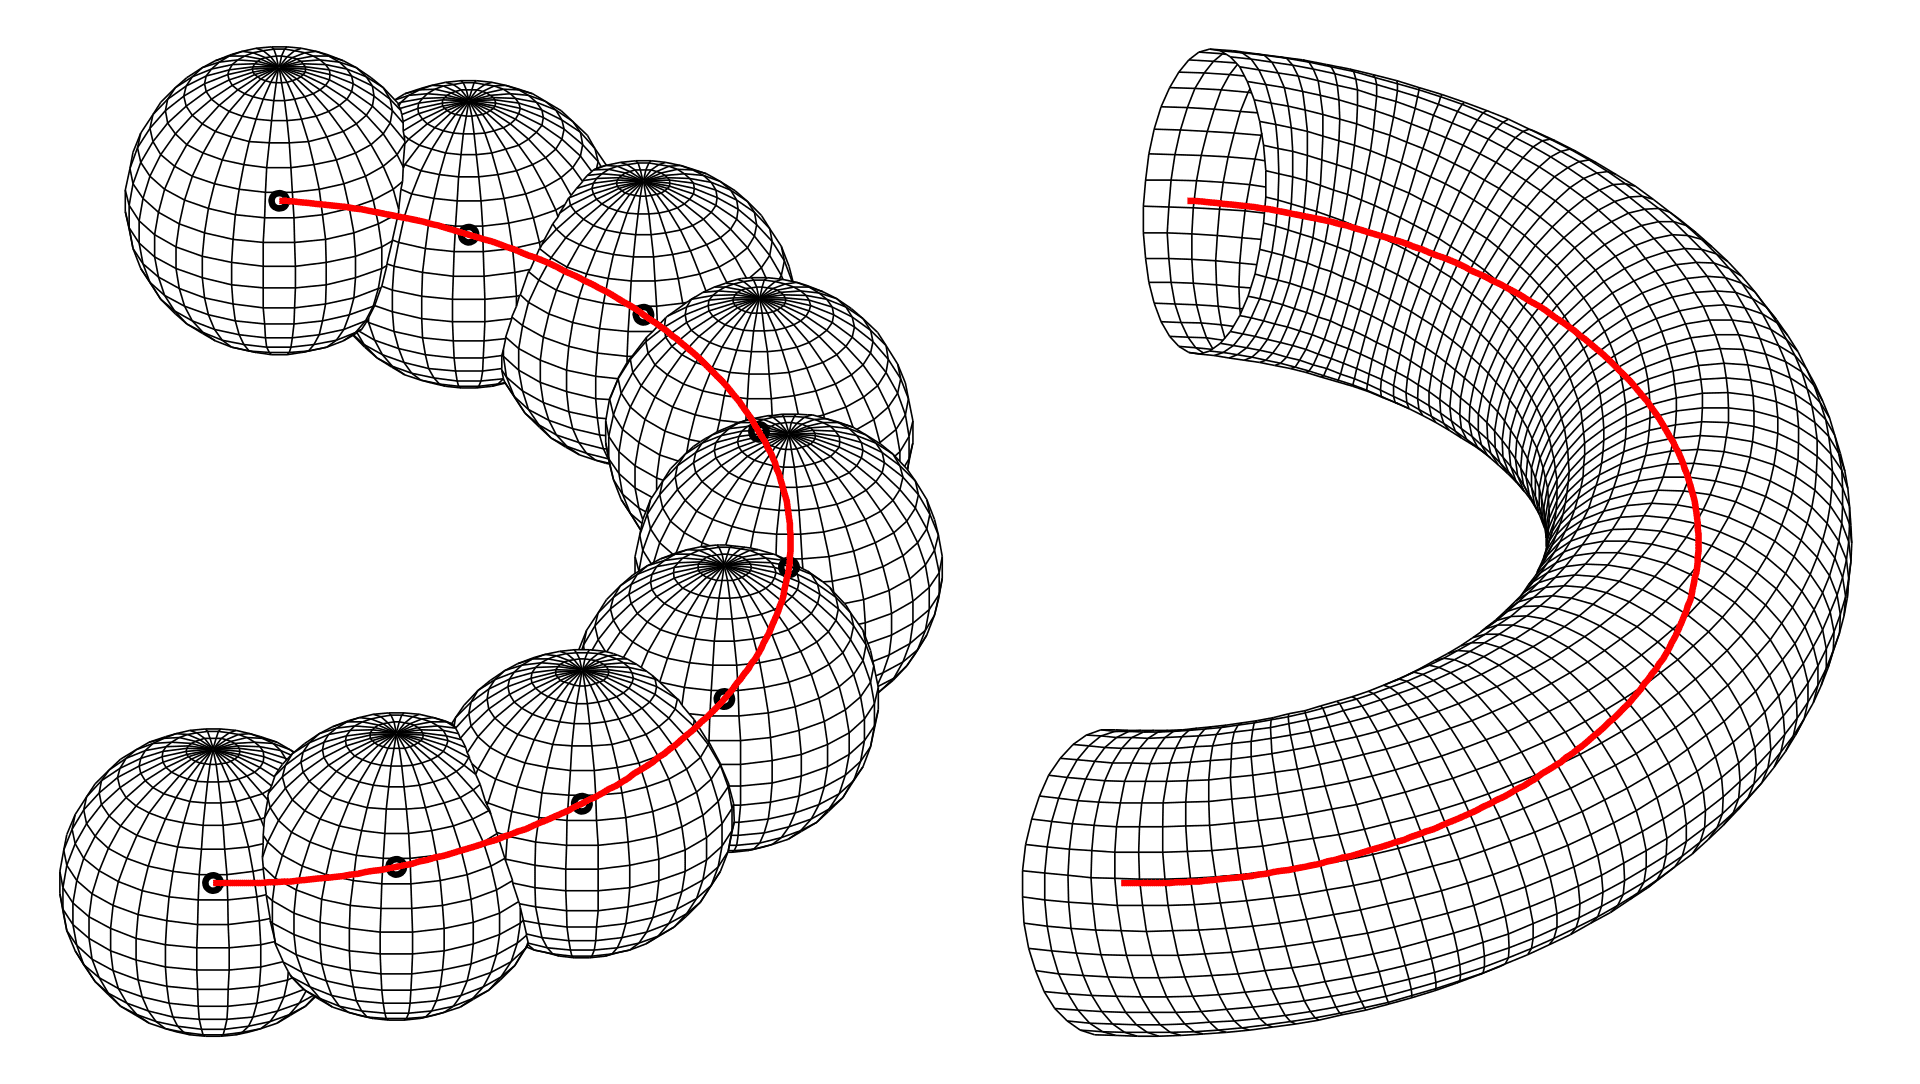
\includegraphics[width=0.7\linewidth]{Images/Channel_Construction.png}
    \caption{Channel as a sweep of sphere}
    \label{fig:enter-label}
\end{figure}

A channel is a surface formed as the envelope of a family of spheres, each with its center on a space curve called the directrix. We’ll generalize this definition to ellipsoids for our specific case. Channel surfaces in topology are formed by sweeping a sphere along a directrix. The directrix determines whether the channel surface is open or closed.

Examples of channel surfaces include:
\begin{itemize}
    \item Right circular cylinder: When the directrix is a straight line and the radii are constant.
    \item Torus: When the directrix is a circle and the radii are constant.
    \item Right circular cone: When the directrix is a straight line and the radii decrease to zero.
\end{itemize}
We aim to plot a channel in MATLAB using two directrices as focal points of rotational ellipsoids. We assume that the two axes other than the focal axis are equal (b = c), which we will refer to as the minor axis or axes. We are provided with a list of discrete position coordinates for the two directrices and the corresponding lengths of either the semi-major or the semi-minor axis.
\[F_{1} = \left\{ \left( p_{i} , q_{i} , r_{i} \right) \right\}\]
\[F_{2} = \left\{ \left( u_{i} , v_{i} , w_{i} \right) \right\}\]
\[A = \left\{ a_{i} \right\} ,or, B = \left\{ b_{i} \right\}\]

\subsection{Matlab Code}
Data is stored in a MATLAB readable text file in seven rows for
\(p,\ q,\ r,\ u,\ v,\ w,a\ or\ b\)

To plot a surface in MATLAB, we use \(surf(x,y,z)\) where
\(x\ ,\ y\ ,\ z\) are matrices of \(2^{nd}\) order and dimensions
\(m \times n\).

\[\begin{bmatrix}
\left( x_{11} ,  y_{11} ,  z_{11}  \right) & \cdots & \cdots & \left( x_{1n} ,  y_{1n} ,  z_{1n}  \right) \\
 \vdots & \ddots & \ddots & \vdots \\
 \vdots & \ddots & \ddots & \vdots \\
\left(  x_{m1} , y_{m1} ,  z_{m1}  \right) & \cdots & \cdots & \left(  x_{mn} , y_{mn} , z_{mn}  \right) \\
\end{bmatrix}\]

\begin{figure}[h]
    \centering
    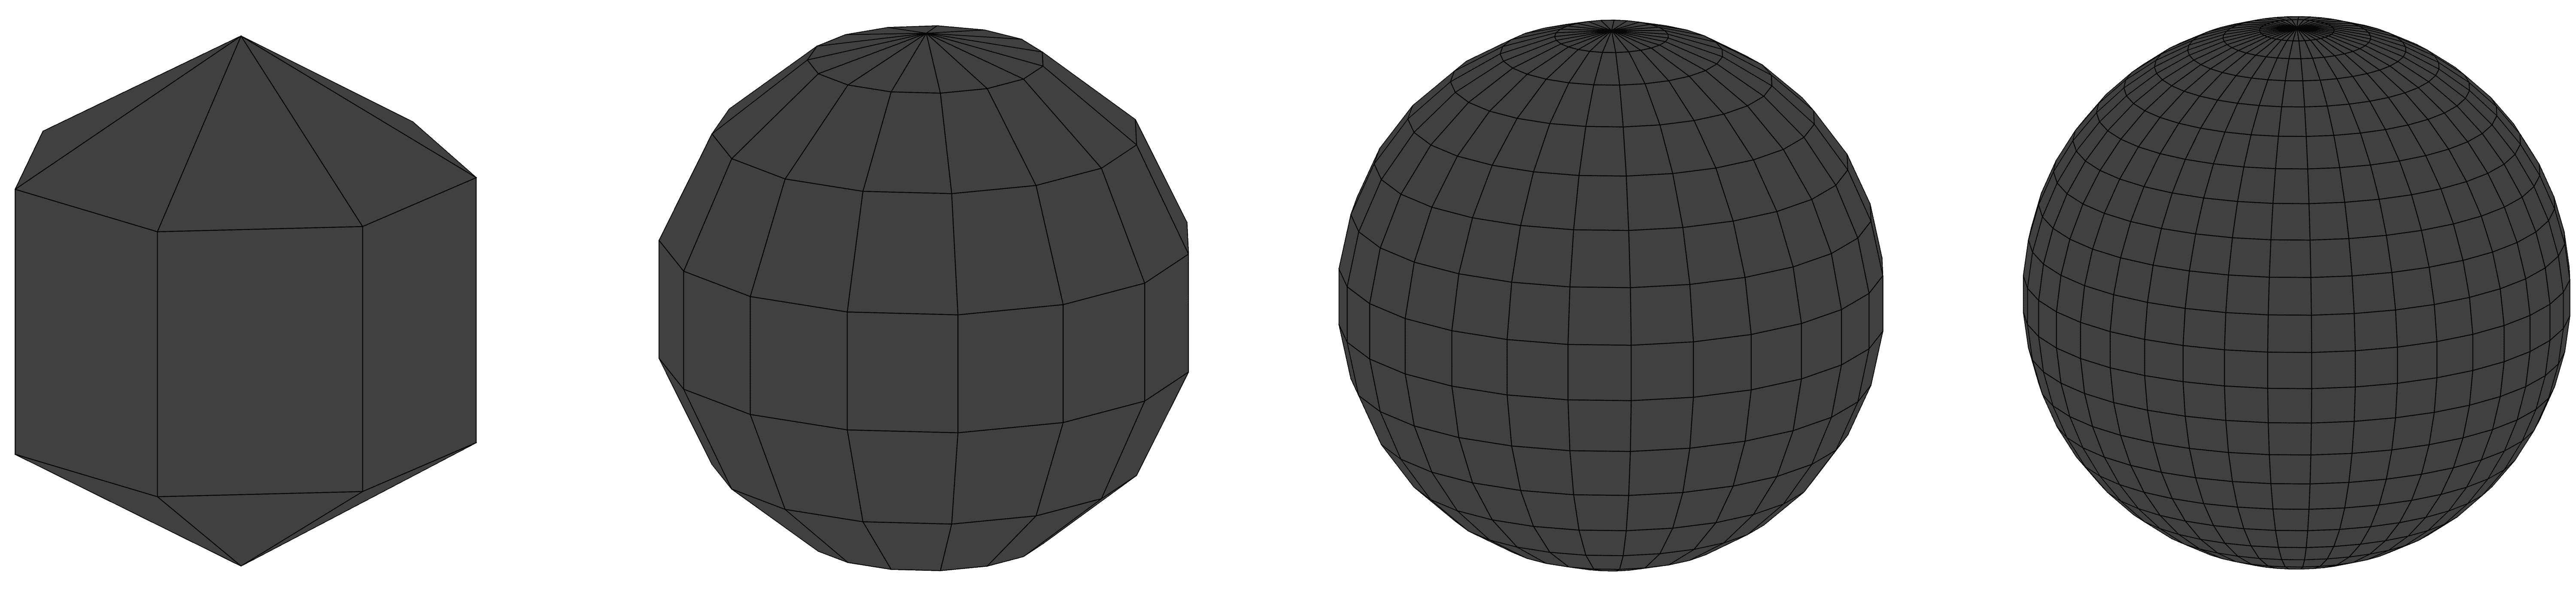
\includegraphics[width=\linewidth]{Images/Sphere_Mesh_Black.png}
    \caption{Sphere as mesh of various densities}
\end{figure}

A “sheet” of points, used by MATLAB to create a mesh of a surface for plotting, consists of columns and rows that form intersecting curves that create a net, which MATLAB fills.

If the data is stored in MATLAB-readable format in a text file, such as “curves.txt”, we can use the \(load()\) function to extract all the data into a variable and then distribute it among various variables.
\\
\begin{lstlisting}[language=matlab]
impdata = load("curves.txt","~ascii");
p   = impdata(1,:);
q   = impdata(2,:);
r   = impdata(3,:);
u   = impdata(4,:);
v   = impdata(5,:);
w   = impdata(6,:);
minor = impdata(7,:);
clear impdata;

\end{lstlisting}
\hypertarget{the-channel-and-the-cylinder}{%
\subsection{The Channel and The
Cylinder}\label{the-channel-and-the-cylinder}}

To simplify the mathematics of a channel, we will make an analogy to one of its special case, A Right Cylindrical Surface.

A Right Cylindrical Surface is a channel formed by a series of spheres, with their directrix being a line. Alternatively, a Solid Cylinder can be thought of as the result of integrating circular discs oriented perpendicular to the directrix. A Cylindrical Surface, on the other hand, is the result of integrating circles or the perimeters of the discs.

\begin{figure}[h]
    \centering
   % 
\includegraphics[width=\linewidth]{Images/Cylinder_Stacks.png}
   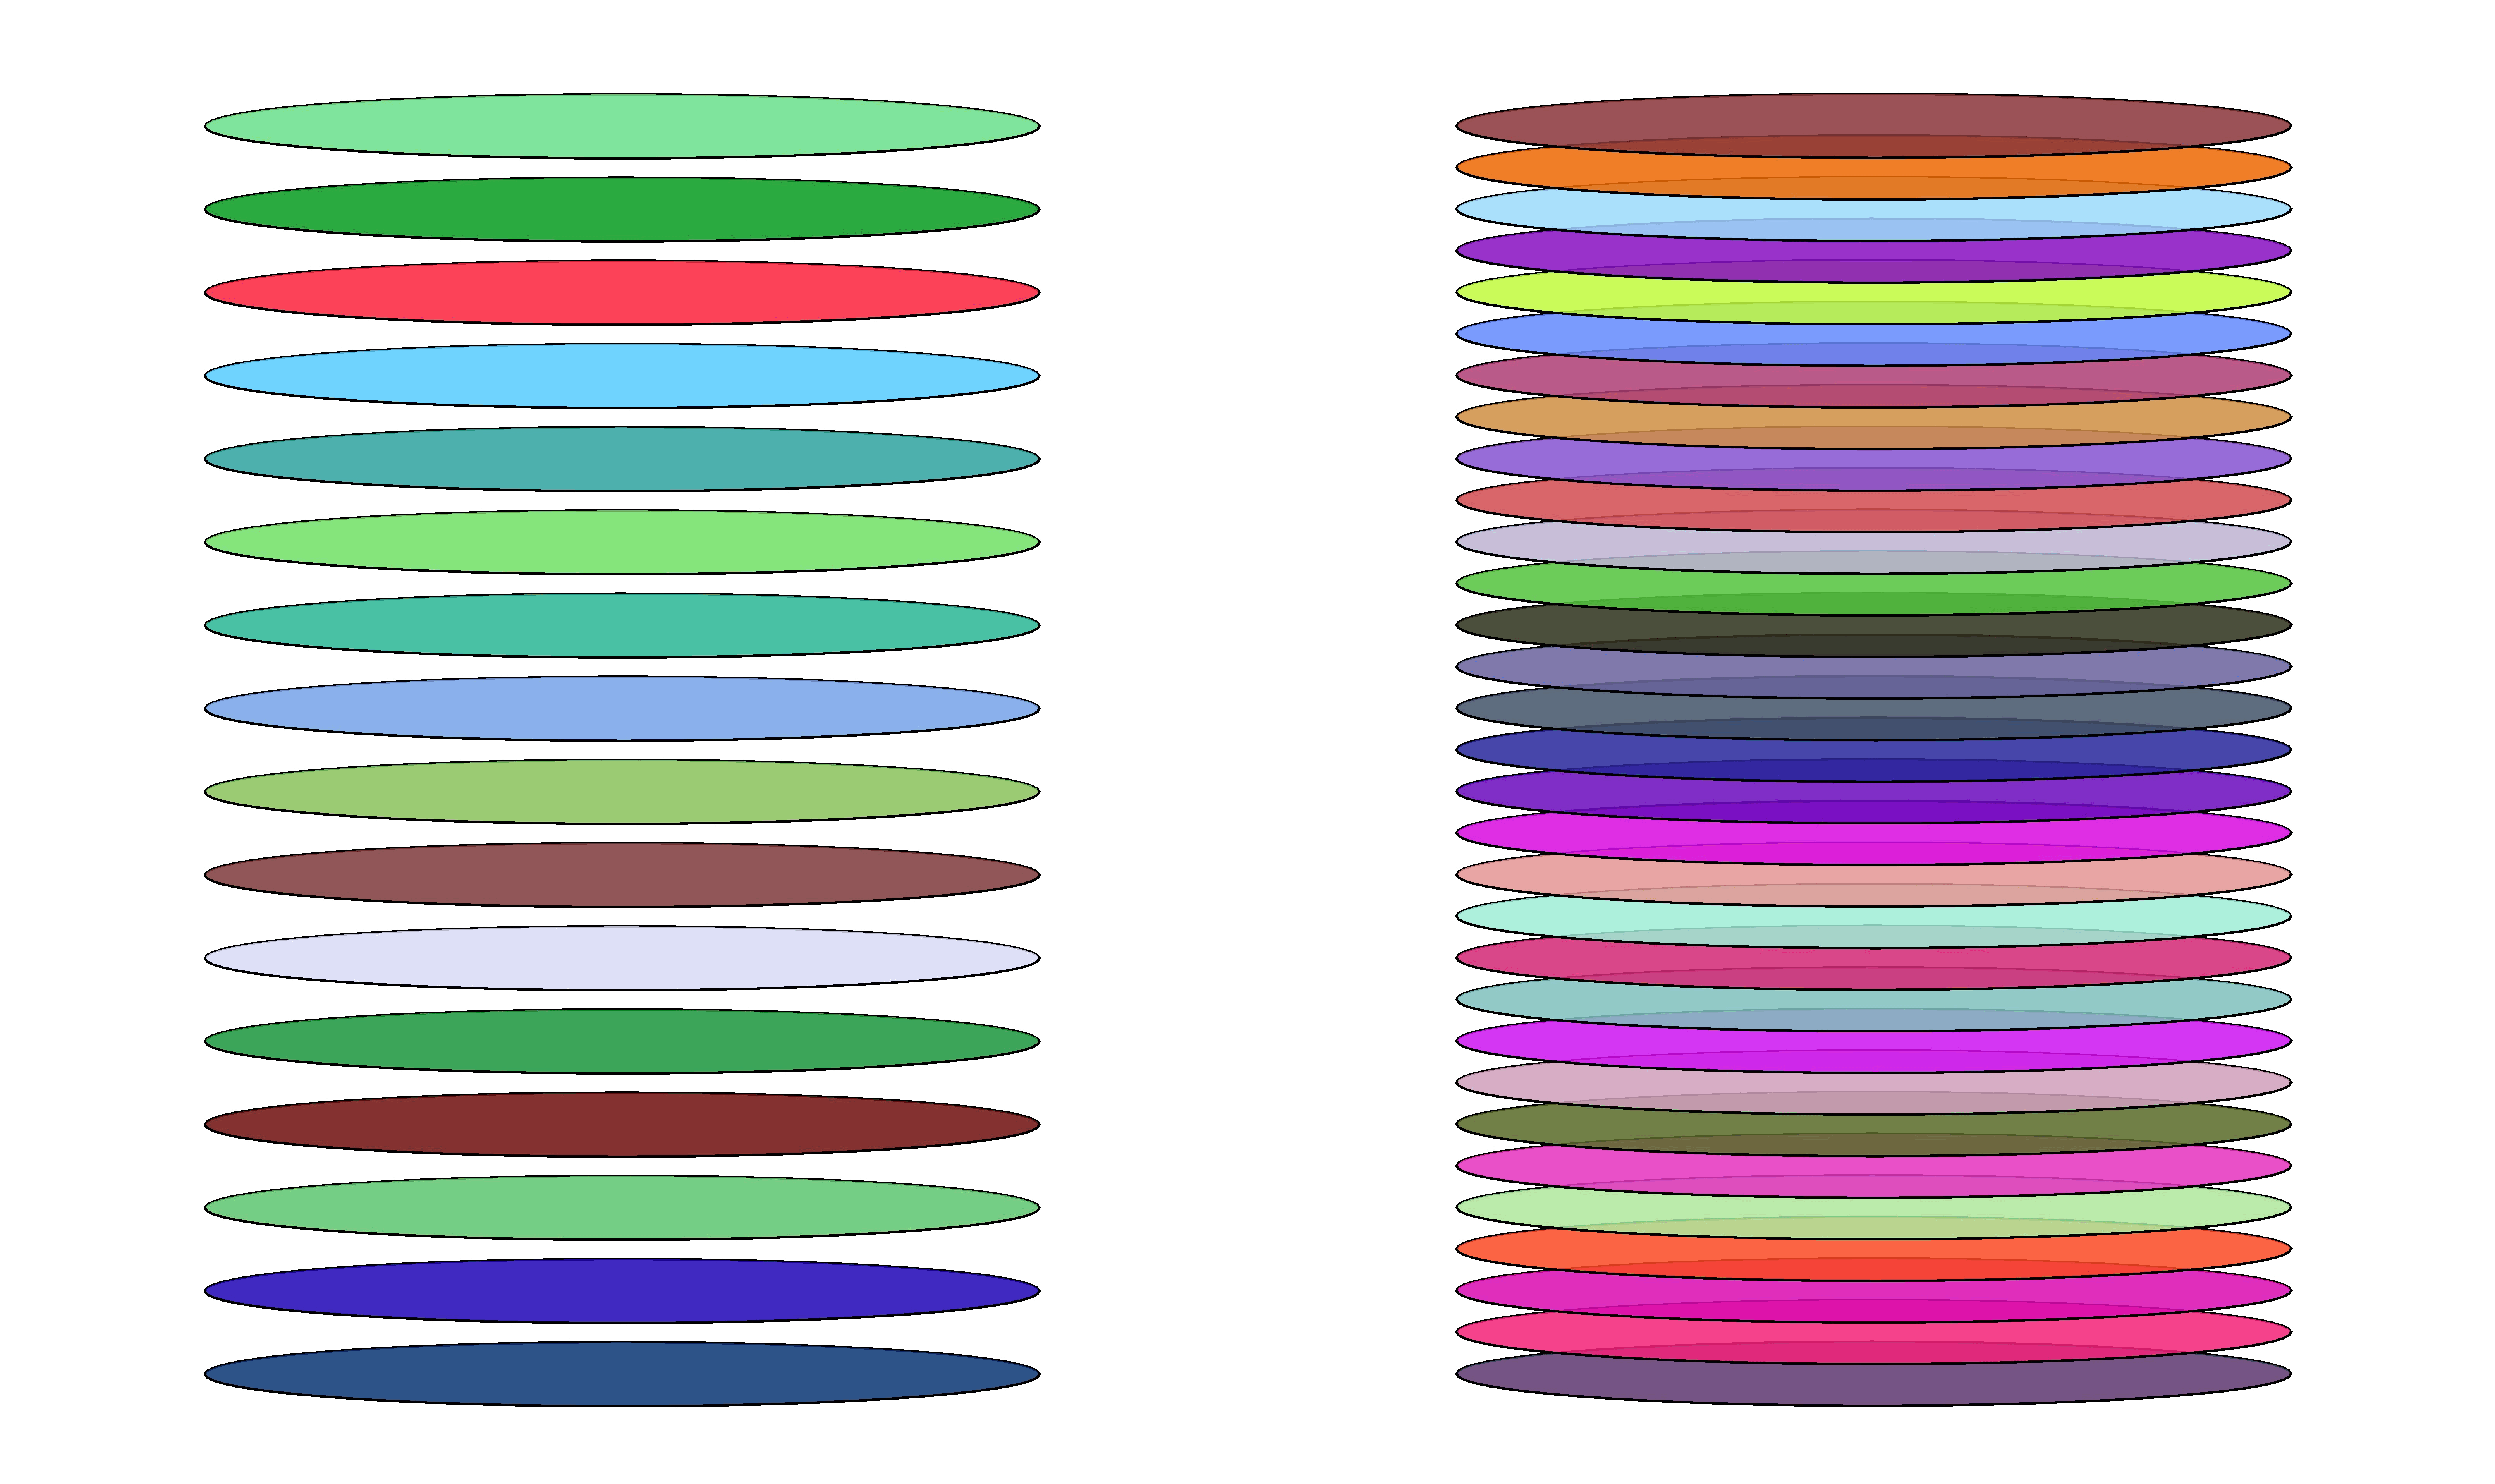
\includegraphics[width=0.7\linewidth]{Images/Cylinder_Stack_Left.jpeg}
   % \subfigure{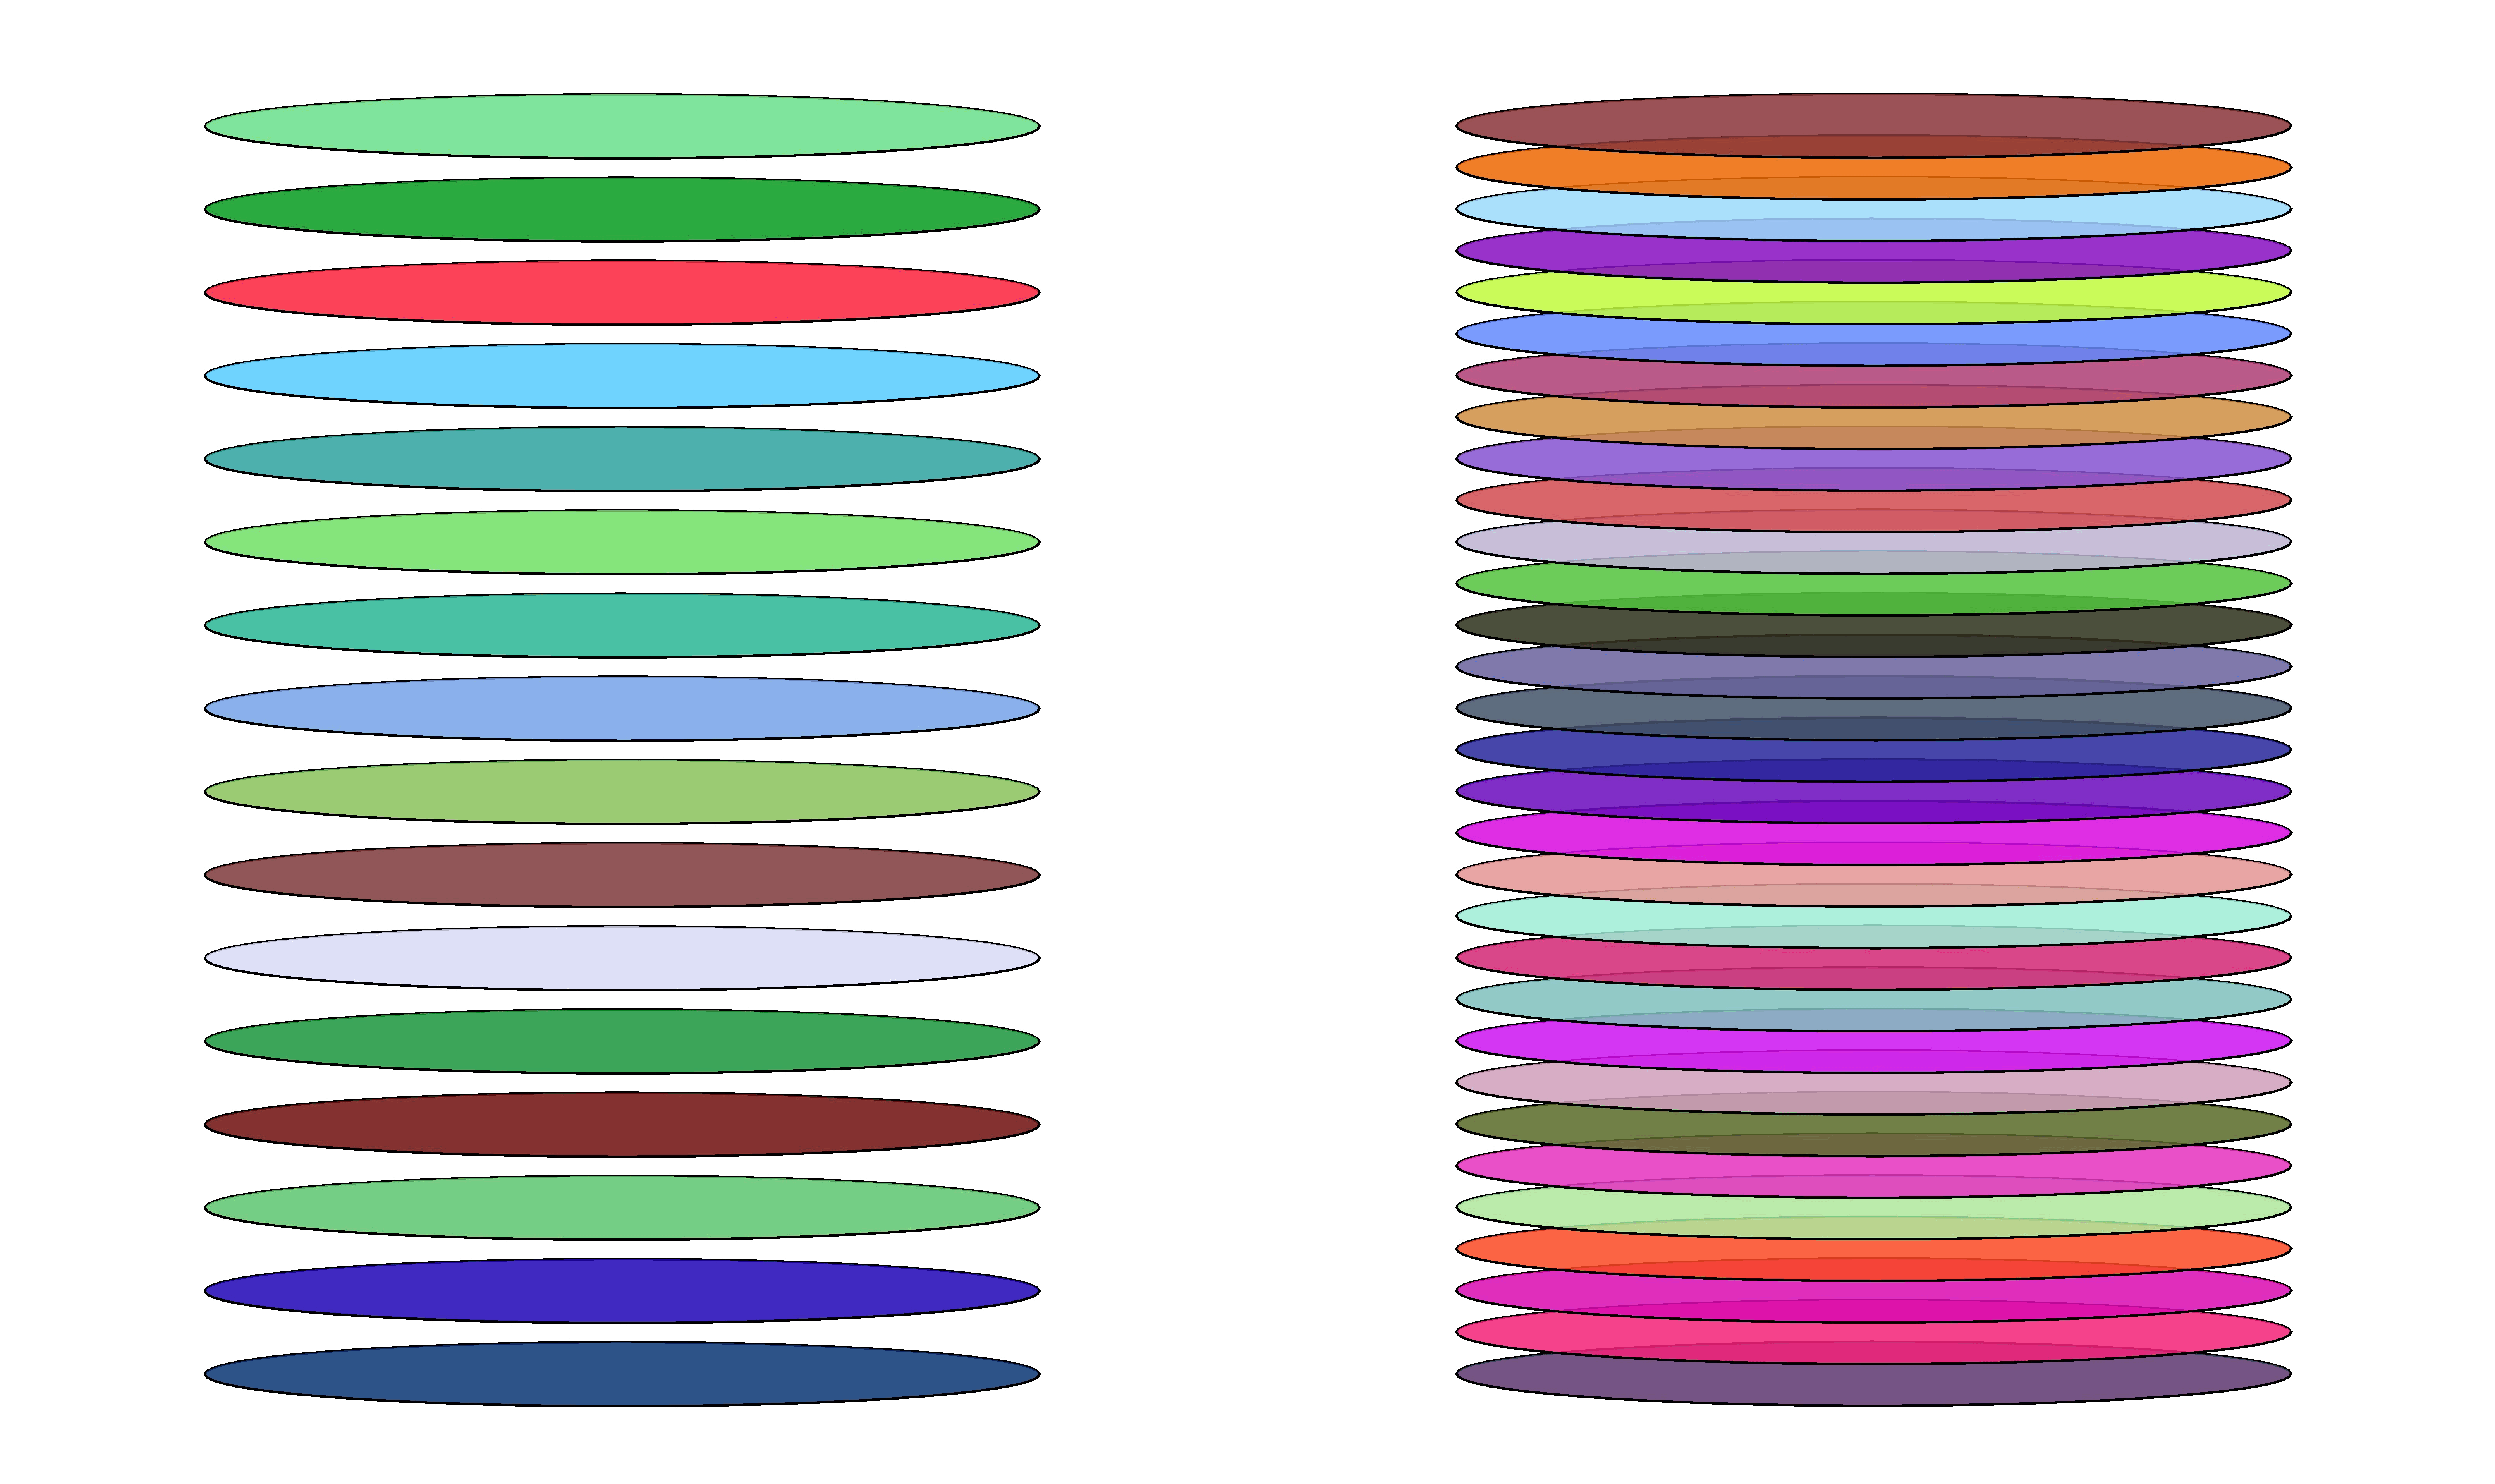
\includegraphics[width=0.8\textwidth]{Images/Cylinder_Stack_Left.jpeg}}
   
    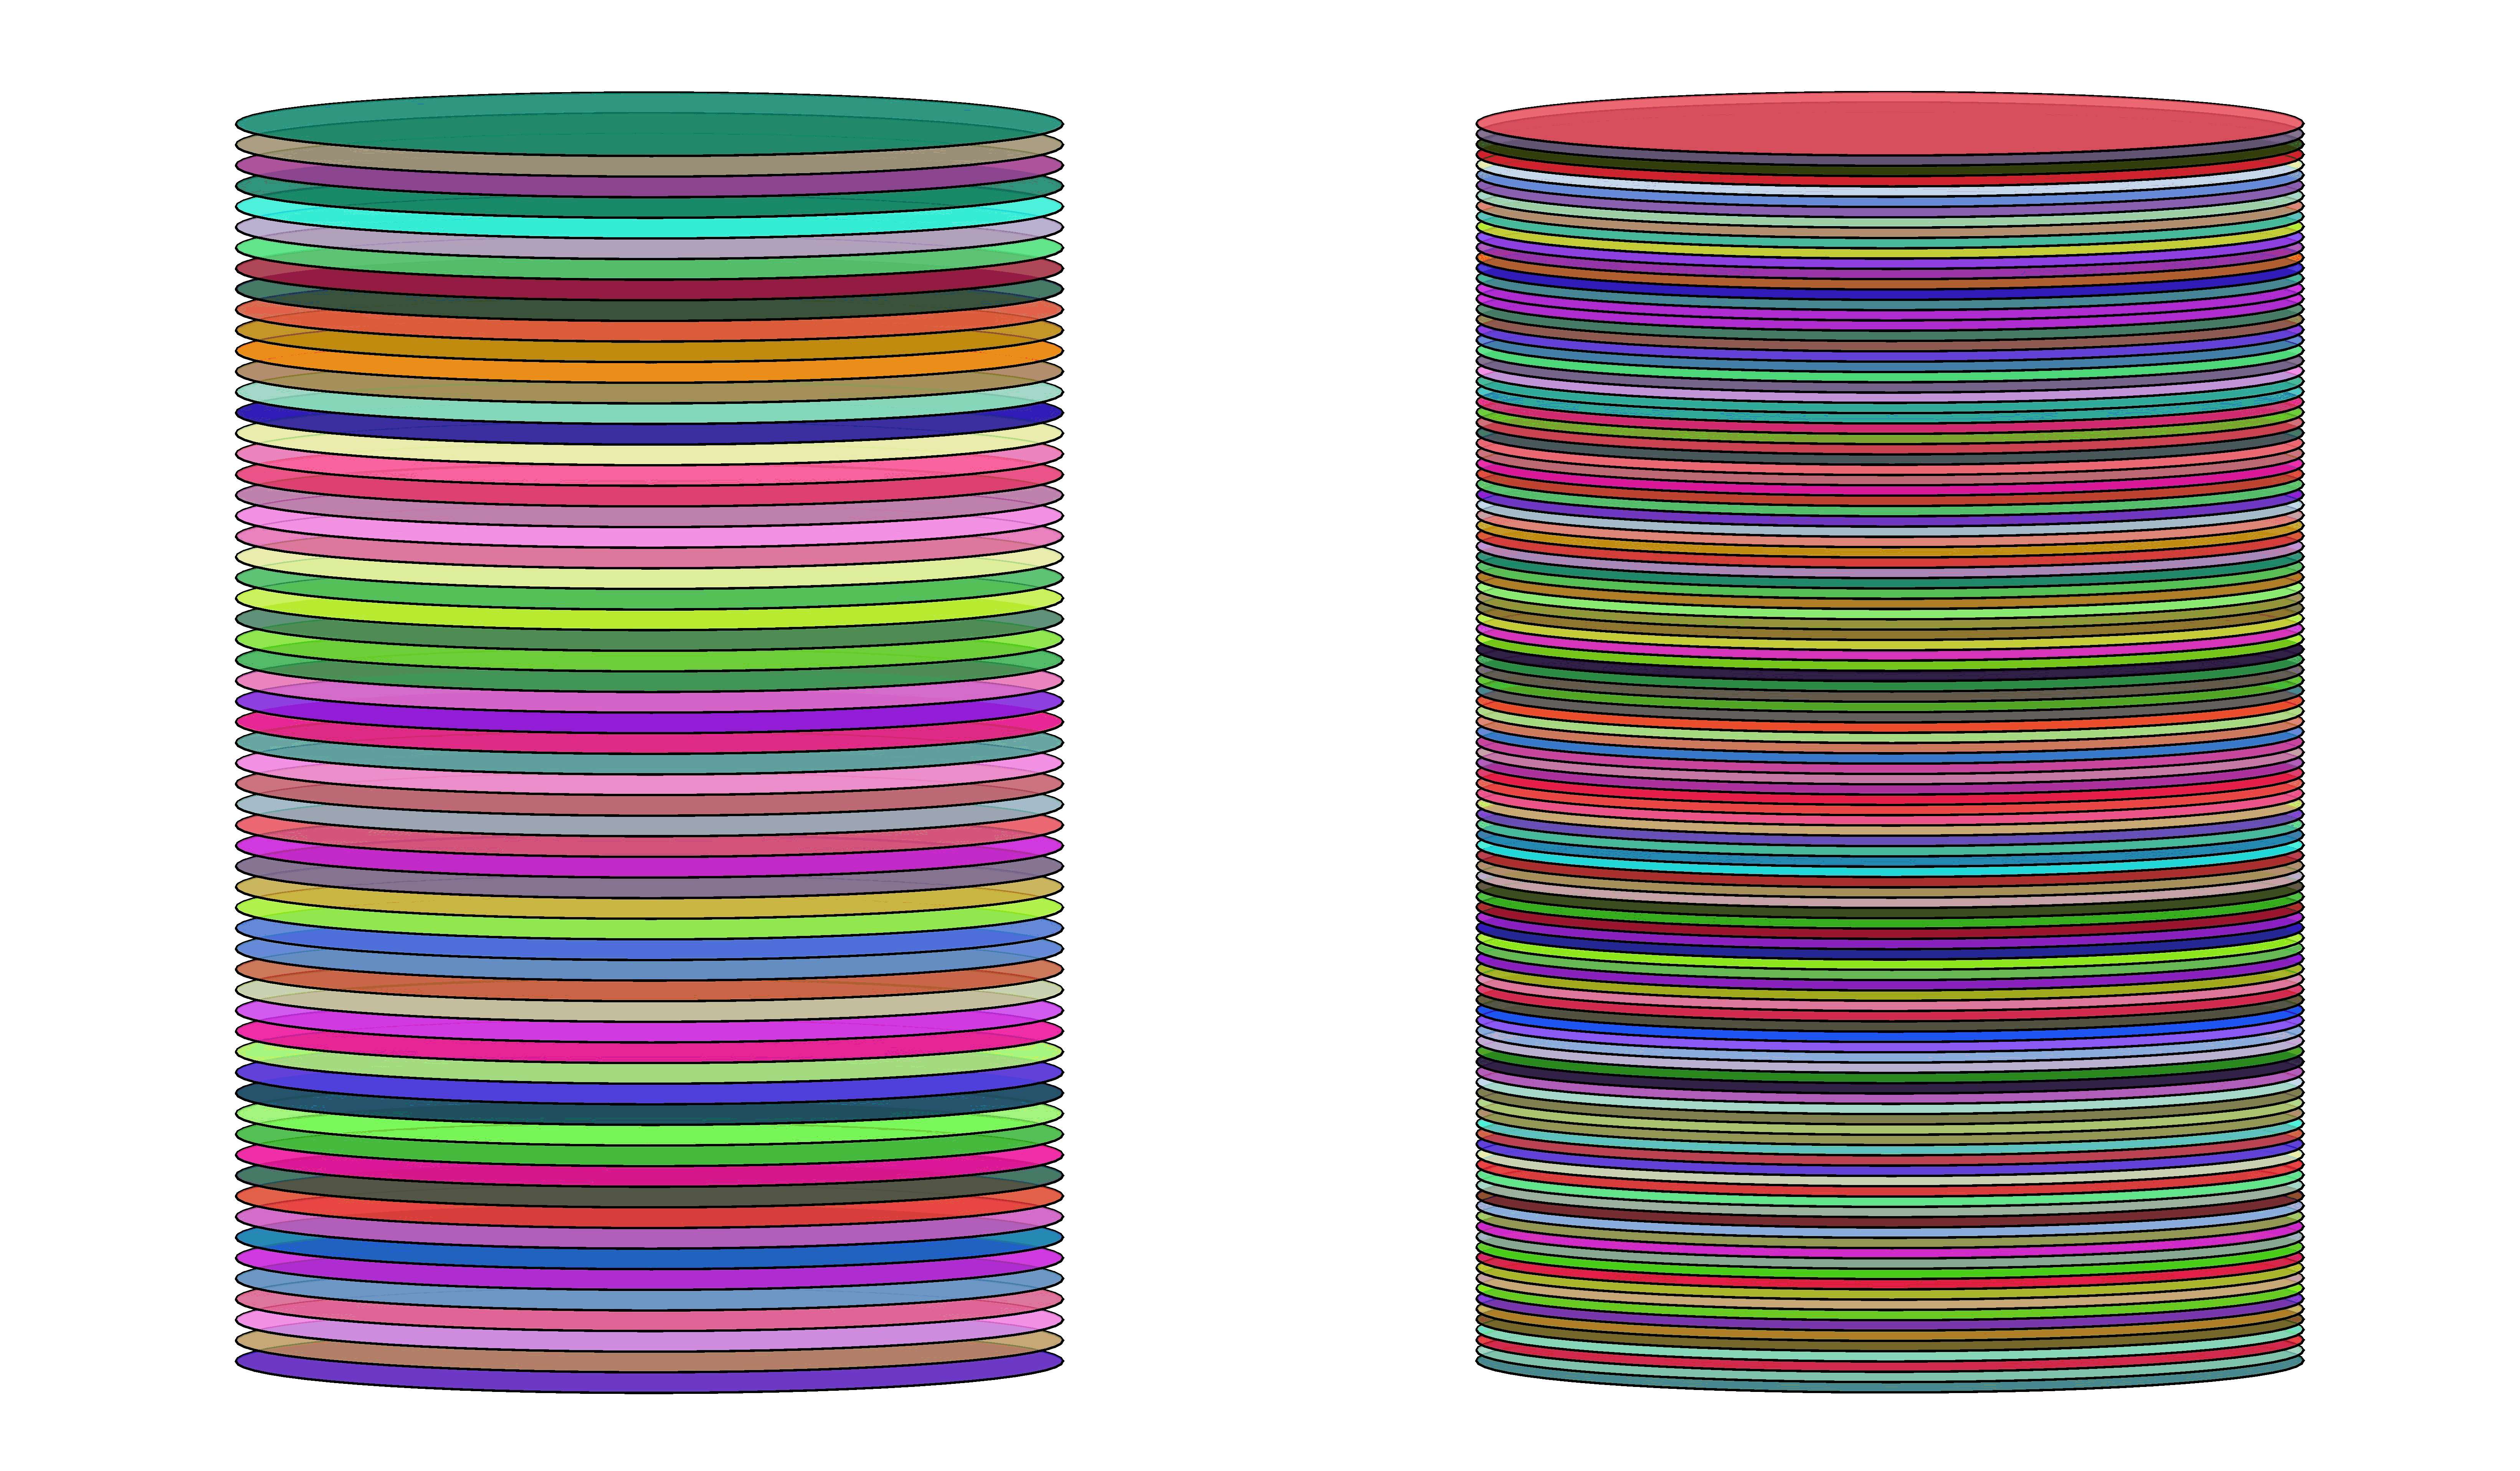
\includegraphics[width=0.72\linewidth]{Images/Cylinder_Stack_Right.jpeg}
  %  \subfigure{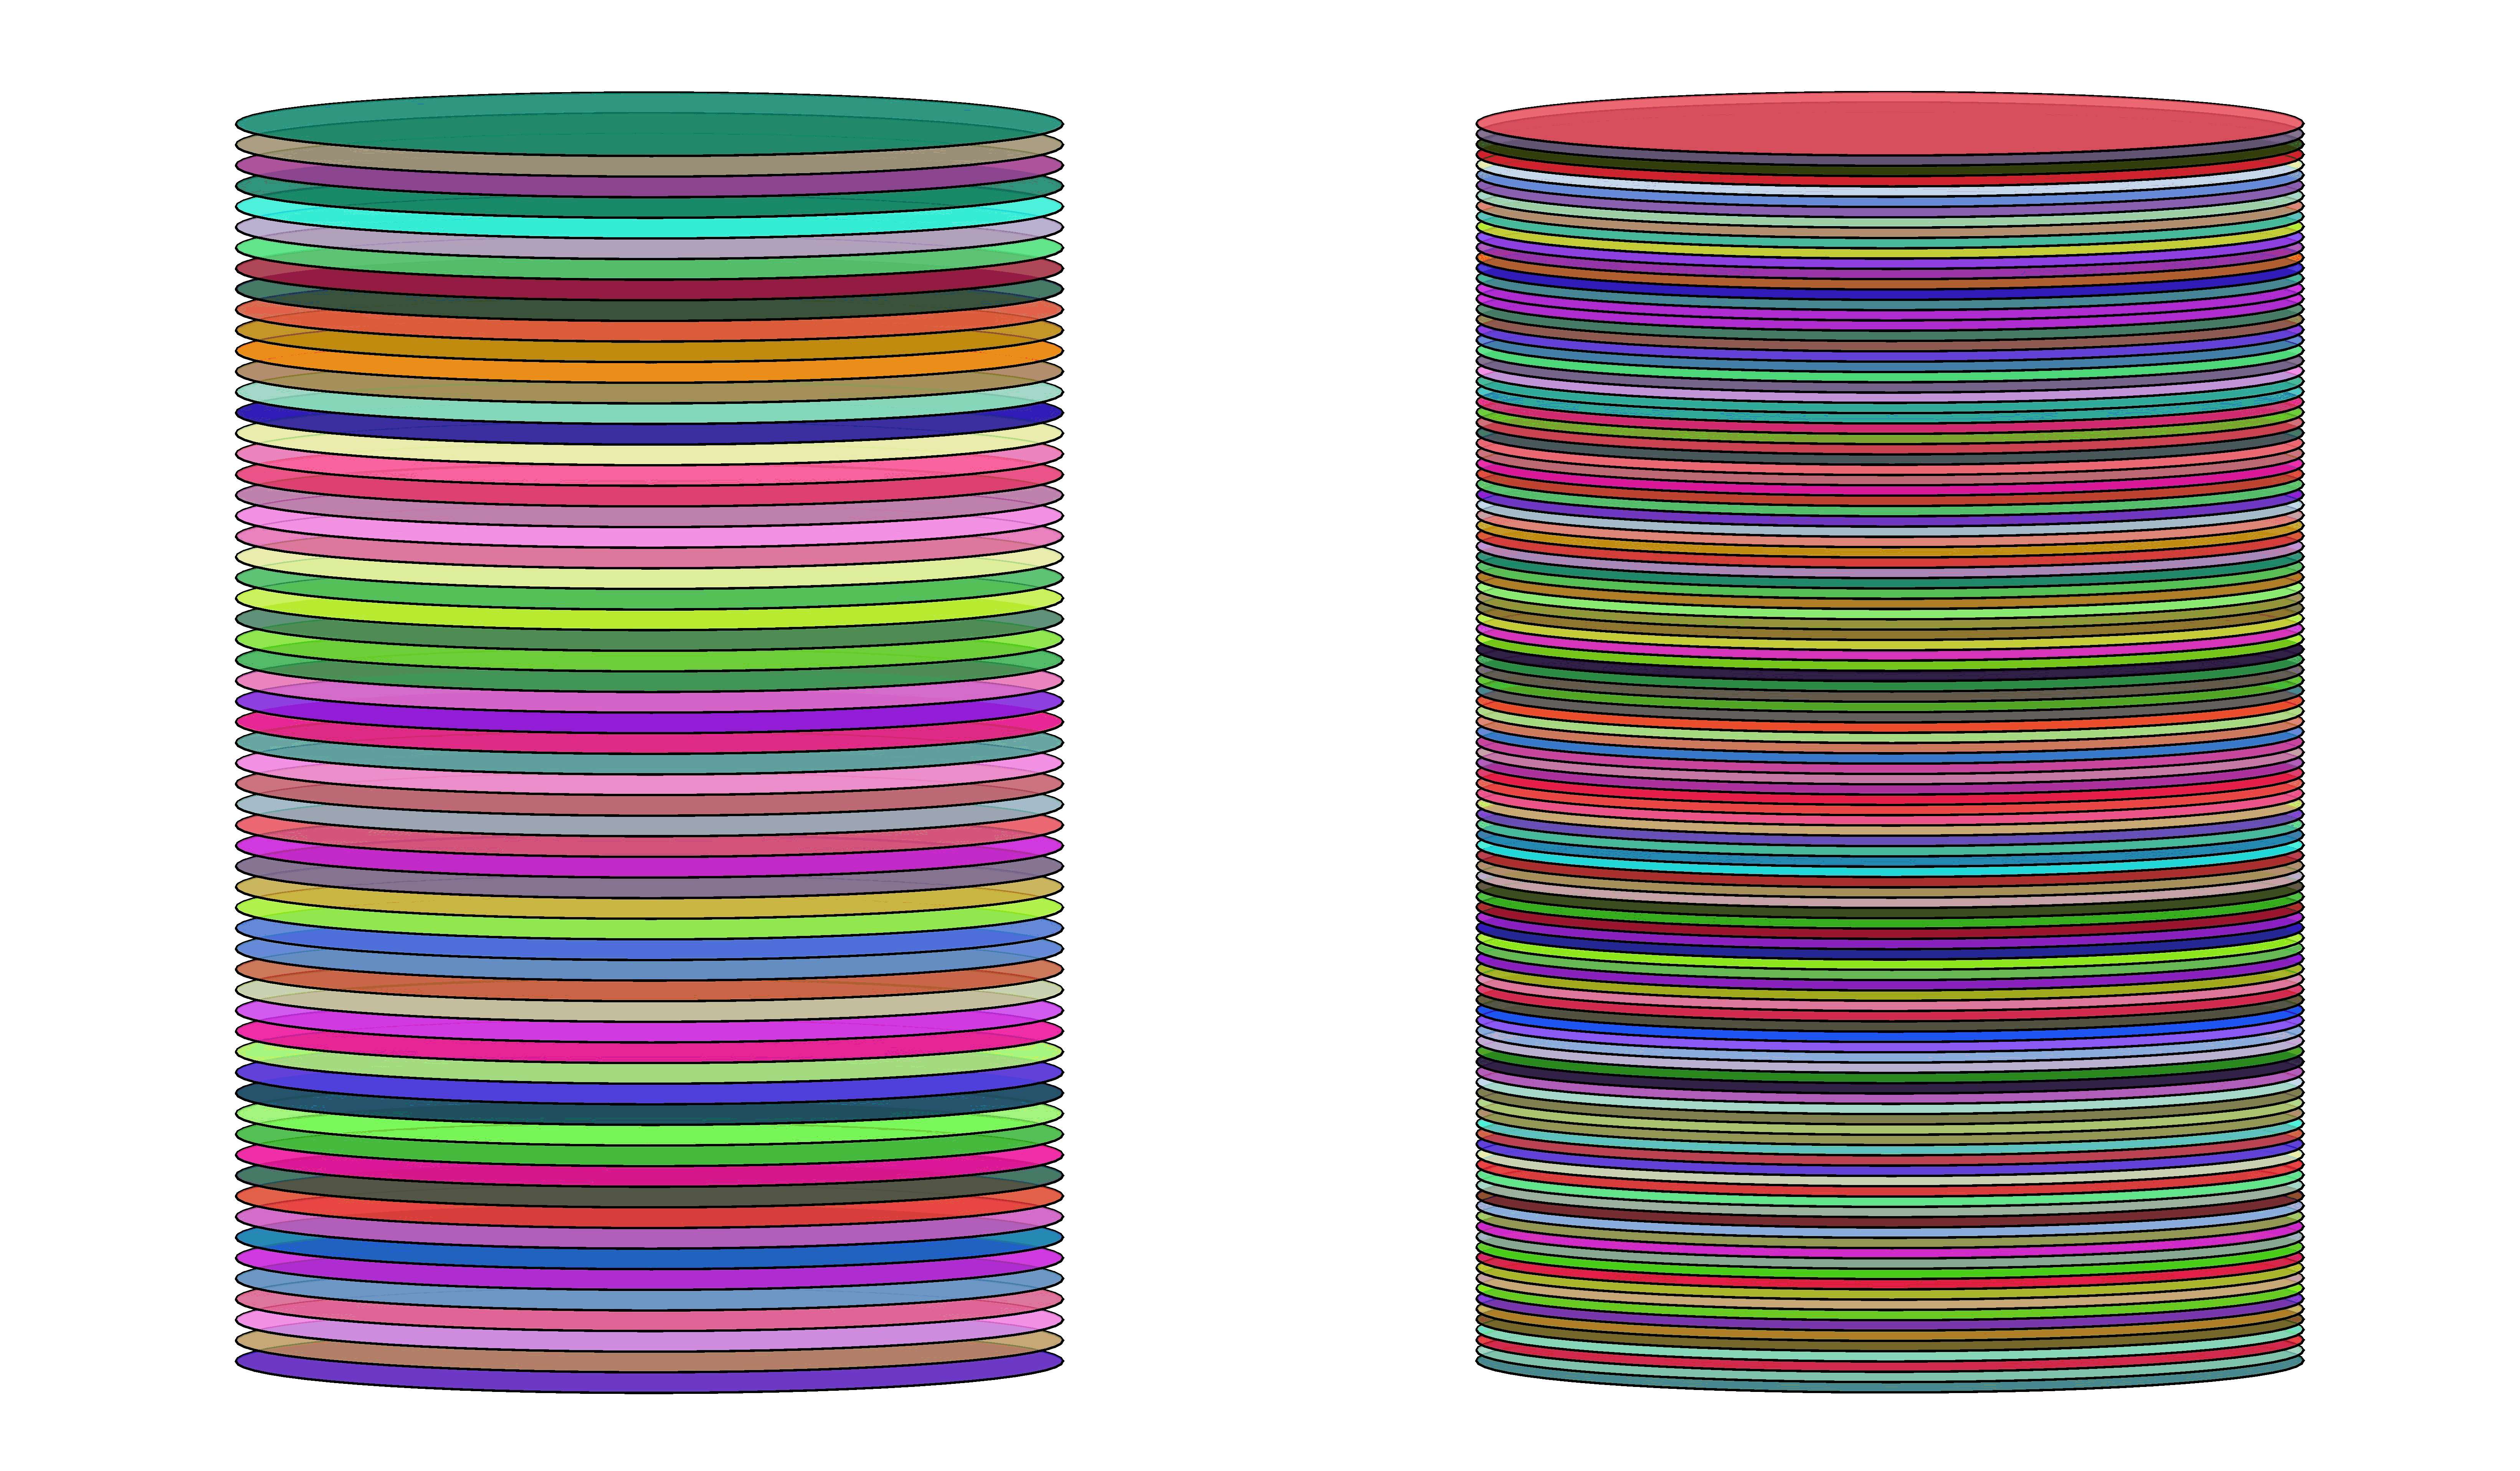
\includegraphics[width=0.8\textwidth]{Images/Cylinder_Stack_Right.jpeg}}
    \caption{Cylinder as Integration of Circular Sheets}
\end{figure}

We can visualize a channel as a cylinder with varying cross-sectional radii. This allows us to calculate the position of points on elliptical cross-sections to create a mesh of the channel.
\newpage
\hypertarget{the-tangents}{%
\section{The Tangents}\label{the-tangents}}

After calculating the Directrix,

\[D = \frac{F_{1} + F_{2}}{2}\]

We are provided with a minor axis length as well, so we will also
determine focal length \& Directrix co-ordinates, and calculate major
axis length.

\begin{lstlisting}[language=matlab]
focal = sqrt( (p-u).^2 + (q-v).^2 + (r-w).^2)\2;
major = sqrt(focal.^2 + minor.^2);

x=(p+u)/2;
y=(q+v)/2;
z=(r+w)/2;
\end{lstlisting}
By default, MATLAB attempts to perform matrix operation on arrays, that is using multiplication and squaring results in matrix multiplication. Therefore, operations are modified with ``\verb|.|" to make them an element-wise operation. ``\verb|.^2|" results in squaring of each element individually, instead of the matrix as a whole. \verb|sqrt()| applies element-wise only.

We have one more necessary parameter to determine: the tangents of directrix. Since we are dealing with a set of discrete points, there are a few techniques that we can use for calculating tangents.
\[\Vec{R}  =  \left(\, x(t)\,  ,\,  y(t) \, , \,  z(t)\, \right)\]

A one dimensional object, like a line or a curve, suspended in a three dimensional space can be represented as each coordinate being a function some independent parameter $'t'$.

Slope is given by:\[  \Vec{M}  =  \left(\, \frac{\partial x}{\partial t} \, ,\,  \frac{\partial y}{\partial t}\,  ,\,  \frac{\partial z}{\partial t}\, \right) \]

If \(t := x\),
\[\Vec{R}  =  \left( \,x\,  ,\,  y(x) \, ,\,  z(x) \,\right)\]

\[  \Vec{M}  =  \left( \,1 \, ,\,  \frac{\partial y}{\partial x}  \,,\,  \frac{\partial z}{\partial x}\, \right) \]
\pagebreak
\hypertarget{global-fit}{%
\subsection{Global Polynomial Fit}\label{GlobalFit}}
Global polynomial fitting involves approximating a dataset using a single polynomial equation of degree $k$ that best represents the data. Once fitted, the polynomial can be differentiated to compute derivatives (e.g., slopes) at any given data point.

Evaluating the slope of a curve can be quite tedious to code. First, we need to determine the coefficients of the fitted polynomial and then use these coefficients to calculate the derivative of the polynomial at each point. Fortunately, we can simplify this process by using MATLAB’s built-in functions. The function \verb|polyfit(x,y,k)| fits the polynomial equation, while the function \verb|polyder(func)| provides the derivative equation \cite{mathworks_polyfit}\cite{mathworks_polyder} . The equation is presented as a row vector, with each element corresponding to a coefficient. Finally, the function \verb|polyval(func,val)| evaluates the value of a polynomial at a specified point \cite{mathworks_polyval}.

\begin{lstlisting}[language=matlab]
% Degree of the polynomial fit
polynomial_order = 3;  % Choose based on the complexity of the data

% Number of points in the dataset
count = size(x, 2);

% Fit polynomials globally for y and z
p_y = polyfit(x, y, polynomial_order);  % Polynomial coefficients for y
p_z = polyfit(x, z, polynomial_order);  % Polynomial coefficients for z

% Compute the derivative coefficients
dp_y = polyder(p_y);  % Derivative coefficients for y
dp_z = polyder(p_z);  % Derivative coefficients for z

% Initialize arrays to store tangents (derivatives) at each point
tangent_y = zeros(1, count);
tangent_z = zeros(1, count);

% Evaluate the derivative polynomials at each point in x
for n = 1:count
    tangent_y(n) = polyval(dp_y, x(n));  % Derivative of y at x(n)
    tangent_z(n) = polyval(dp_z, x(n));  % Derivative of z at x(n)
end
\end{lstlisting}

\subsubsection*{Operational Complexity}
\begin{itemize}
    \item \textbf{Polynomial Fitting (\texttt{polyfit}):} 
    \[O(n \cdot k + k^3),\]
     where \( n \) is the number of points and \( k \) is the degree of the polynomial.\\
    The cubic term \( O(k^3) \) dominates due to solving the linear system.

    \item \textbf{Derivative Computation (\texttt{polyder}):}
    \[O(k)\] for each polynomial.
    This step is negligible compared to the others.

    \item \textbf{Polynomial Evaluation (\texttt{polyval})}:
    \[O(n \cdot k)\]
    as the derivative polynomial is evaluated at all \( n \) points.
\end{itemize}

\textbf{Total Complexity:} \(O(n \cdot k + k^3)\)

\paragraph*{Key Observations}
\begin{itemize}
    \item For large \( n \), the term \( O(n \cdot k) \) dominates.
    \item For large \( k \), the cubic cost \( O(k^3) \) from \texttt{polyfit} dominates.
    \item The code is efficient for small \( k \) but becomes computationally expensive for high-degree polynomials.
\end{itemize}

\subsubsection{Limitations}
This runs the risk of either overestimating or underestimating the curve if proper degree of the polynomial is not used. This requires prior understanding of expected behaviour of the data. While the curve itself may follow closely to the data, derivatives may not be so accurate. Caution is advised using this method.

\hypertarget{spline-fit}{%
\subsection{Spline Interpolation}\label{Spline}}

Spline interpolation is a piecewise polynomial method used to approximate a dataset by constructing smooth polynomials between consecutive points. Unlike global polynomial fitting, spline interpolation avoids overfitting and instabilities, making it particularly effective for large datasets or irregularly spaced data.

The most common spline interpolation technique is \textbf{cubic spline interpolation}, which uses cubic polynomials for each interval. For $n$ data points, we construct $n$ polynomials, one for each interval: Spline interpolation is a powerful method for slope and value estimation in datasets where smoothness and accuracy are critical.

\begin{lstlisting}[language=matlab]
window_size = 5;    % Number of points in the fitting window
max_order = 3;      % Maximum degree of the polynomial fit
count = size(x, 2); % Total number of Points

tangent_y = zeros(1, count);
tangent_z = zeros(1, count);

for n = 1:count
    % Determine the indices for the fitting window
    half_window = floor(window_size / 2);
    start_idx = max(1, n - half_window);
    end_idx = min(count, n + half_window);
    
    x_window = x(start_idx:end_idx);
    y_window = y(start_idx:end_idx);
    z_window = z(start_idx:end_idx);
    
    % Determine the polynomial order based on the window size
    current_order = min(max_order, length(x_window) - 1);
    
    p_y = polyfit(x_window, y_window, current_order);
    p_z = polyfit(x_window, z_window, current_order);
    
    dp_y = polyder(p_y);
    dp_z = polyder(p_z);
    
    tangent_y(n) = polyval(dp_y, x(n));
    tangent_z(n) = polyval(dp_z, x(n));
end

\end{lstlisting}

\subsubsection*{Operational Complexity}
\begin{itemize}
    \item \textbf{Polynomial Fitting (\texttt{polyfit})}: 
    \[
    O(m \cdot k^2 + k^3)
    \]
    where \( m \) is the window size and \( k \) is the polynomial degree.
    \item \textbf{Derivative Computation (\texttt{polyder})}:
    \[
    O(k)
    \]
    \item \textbf{Polynomial Evaluation (\texttt{polyval})}:
    \[
    O(k)
    \]
\end{itemize}

\textbf{Cost Per Iteration:} \(O(m \cdot k^2 + k^3)\)

\textbf{Total Complexity:} \(O(n \cdot (m \cdot k^2 + k^3))\)

\paragraph*{Observations}
\begin{itemize}
    \item Complexity scales linearly with \( n \) (number of points) and \( m \) (window size).
    \item The \( k^3 \) term dominates due to the cost of solving the linear system in \texttt{polyfit}.
\end{itemize}

\subsubsection{Limitation}
The \verb|polyfit| function in MATLAB throws an error when the data points are too close to each other, for instance, when the difference between any two consecutive points is less than \(0.01\). Essentially, MATLAB considers data points that are too close to each other to be redundant, as they essentially represent the same point. For such that cases, we can use much a simpler tool.

\hypertarget{Central Finite Difference}{%
\subsection{Central Finite Difference}\label{lagranges-mean-value-theorem}}

\begin{figure}[h]
    \centering
    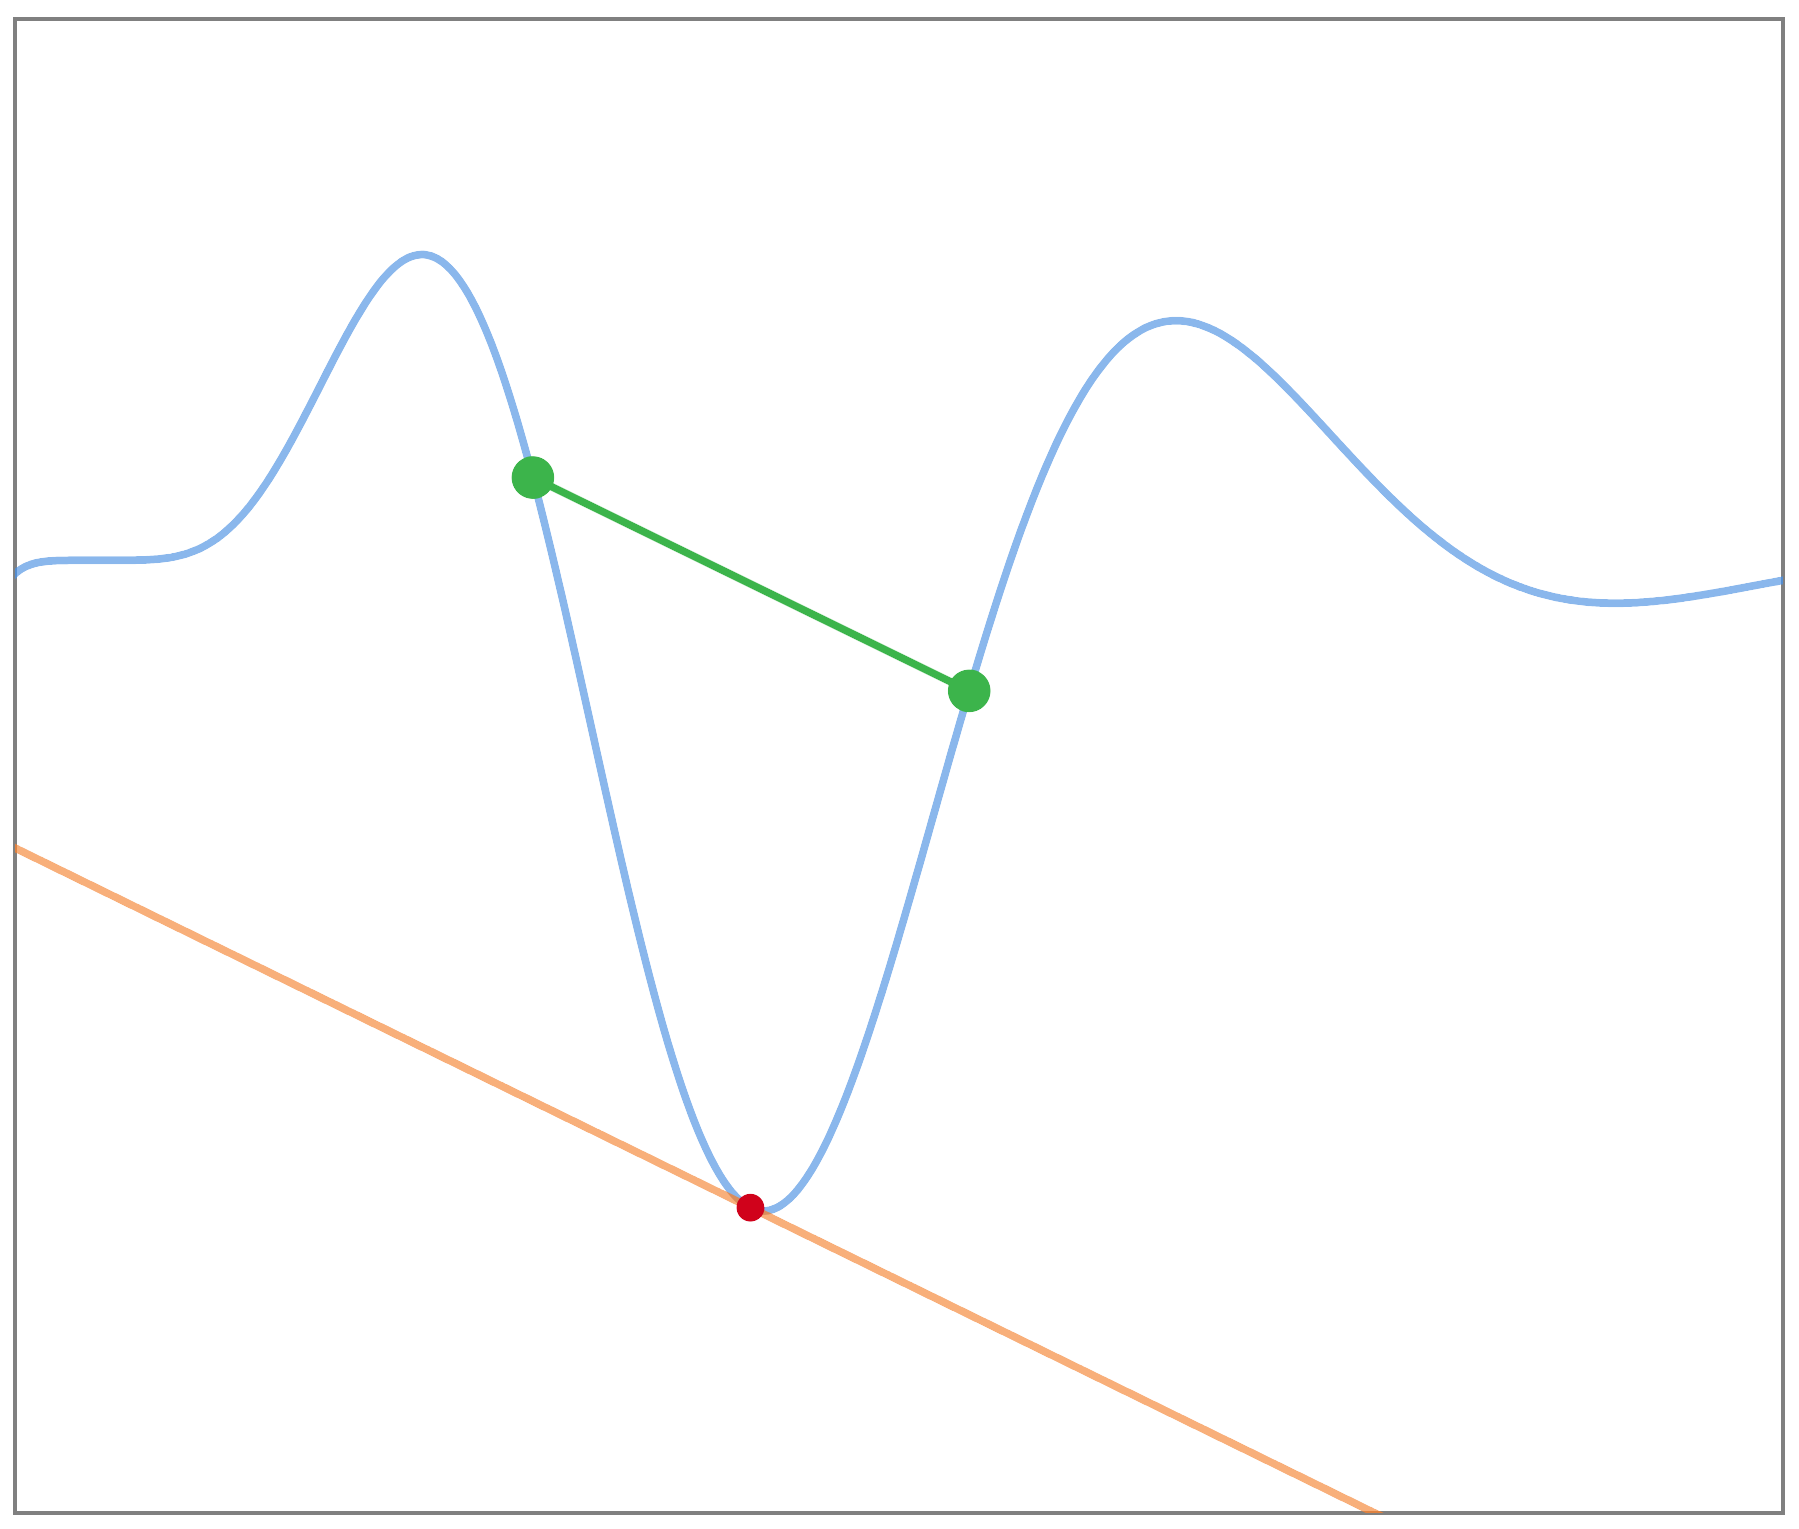
\includegraphics[width=0.5\linewidth]{Images/Mean Value Tangent.jpeg}
    \caption{Line connecting two points is the slope at some point that lies between the given points of the curve they lie on}
\end{figure}
This method is mainly based on Lagrange's mean value theorem that states that in any interval \(\lbrack a,b\rbrack\), there is some \(c\), for which

\[f^{'}(c) = \frac{f(b) - f(a)}{b - a}\]

We assume that the point\(c\) is close enough to our point that we can approximate its tangent as being equal to our point. This approximation becomes more accurate as the boundary points get closer, to the extent that these three points almost form a straight line and our point almost lies on it.
This method is simple, fast, and shines exceptionally bright in the dark shadows of Spline Interpolation.

\[\frac{\partial\vec{R}}{\partial x} = \frac{\partial x}{\partial x}\ \hat{i} + \frac{\partial y}{\partial x}\ \hat{j} + \frac{\partial z}{\partial x}\ \hat{k}\]

\[\frac{\mathrm{\Delta}\vec{R}}{x_{2} - x_{1}} = 1\ \hat{i} + \frac{y_{2} - y_{1}}{x_{2} - x_{1}}\ \hat{j} + \frac{z_{2} - z_{1}}{x_{2} - x_{1}}\ \hat{k}\]

\[\vec{M} = 1\ \hat{i} + \frac{y_{2} - y_{1}}{x_{2} - x_{1}}\ \hat{j} + \frac{z_{2} - z_{1}}{x_{2} - x_{1}}\ \hat{k}\]

\begin{lstlisting}[language=matlab]
count=size(x,2);

tangent_y = zeros(1,count);
tangent_z= zeros(1,count);

tangent_y(1)= (y(2)-y(1))/(x(2)-x(1));
tangent_z(1)= (z(2)-z(1))/(x(2)-x(1));

tangent_y(end)= (y(end)-y(end-1))/(x(end)-x(end-1));
tangent_z(end)= (z(end)-z(end-1))/(x(end)-x(end-1));

for n=2:count-1
    tangent_y(n)=(y(n+1)-y(n-1))/(x(n+1)-x(n-1));
    tangent_z(n)=(z(n+1)-z(n-1))/(x(n+1)-x(n-1));
end

\end{lstlisting}

Spline interpolation excels where finite difference fails and vice versa. These two powerful tools complement each other, filling in the gaps in each other’s capabilities. Either of them can be used modularly depending upon the need of the data
\pagebreak
\subsection{Comparison of Methods}
\begin{table}[ht]
    \centering
    \begin{tabular}{@{}p{0.13\linewidth}p{0.25\linewidth}p{0.27\linewidth}p{0.25\linewidth}@{}}
    \toprule \rule{0pt}{3ex}
    \textbf{} & \textbf{Global Fitting} & \textbf{Spline Fitting} & \textbf{Finite Difference} \rule[-2.5ex]{0pt}{0pt}\\
    \midrule\\
    \textbf{Process} & 
    Fit a single \( k \)-th degree polynomial to all data points, then differentiate. & 
    Fit \( n \) piecewise \( k \)-th degree polynomials, then differentiate each segment. & 
    Use finite differences between neighboring points to estimate derivatives. \\
    \\
    \textbf{Strengths} & 
    Smooth, continuous data; small to medium datasets. & 
    Data with sharp transitions, non-uniform spacing, or local trends requiring adaptive fitting. & 
    Smooth, evenly spaced data where computational efficiency is crucial. \\
    \\
    \textbf{Weaknesses} & 
    Overfitting or instability with high-degree polynomials or large datasets. & 
    Computational cost scales with number of intervals; poor approximation with sparse data; MATLAB issues with too dense data. & 
    Sensitive to noise; unsuitable for uneven spacing or discontinuities. \\
    \\
    \textbf{Complexity} & 
    \( O(nk^2 + k^3) \) & 
    \( O(nk^2 + nk) \) & 
   \( O(n) \)\rule[-2.5ex]{0pt}{0pt}\\
   \bottomrule 
    \end{tabular}
    \caption{Comparison of methods for derivative estimation.}
    \label{tab:comparison}
    \end{table}

Data that we use as test data is very dense and smooth. Therefore, we will use the Central Finite Difference.
\newpage
\hypertarget{the-ellipses}{%
\section{\texorpdfstring{The Ellipses}{ The Ellipses}}\label{the-ellipses}}

\begin{figure}[h]
    \centering
    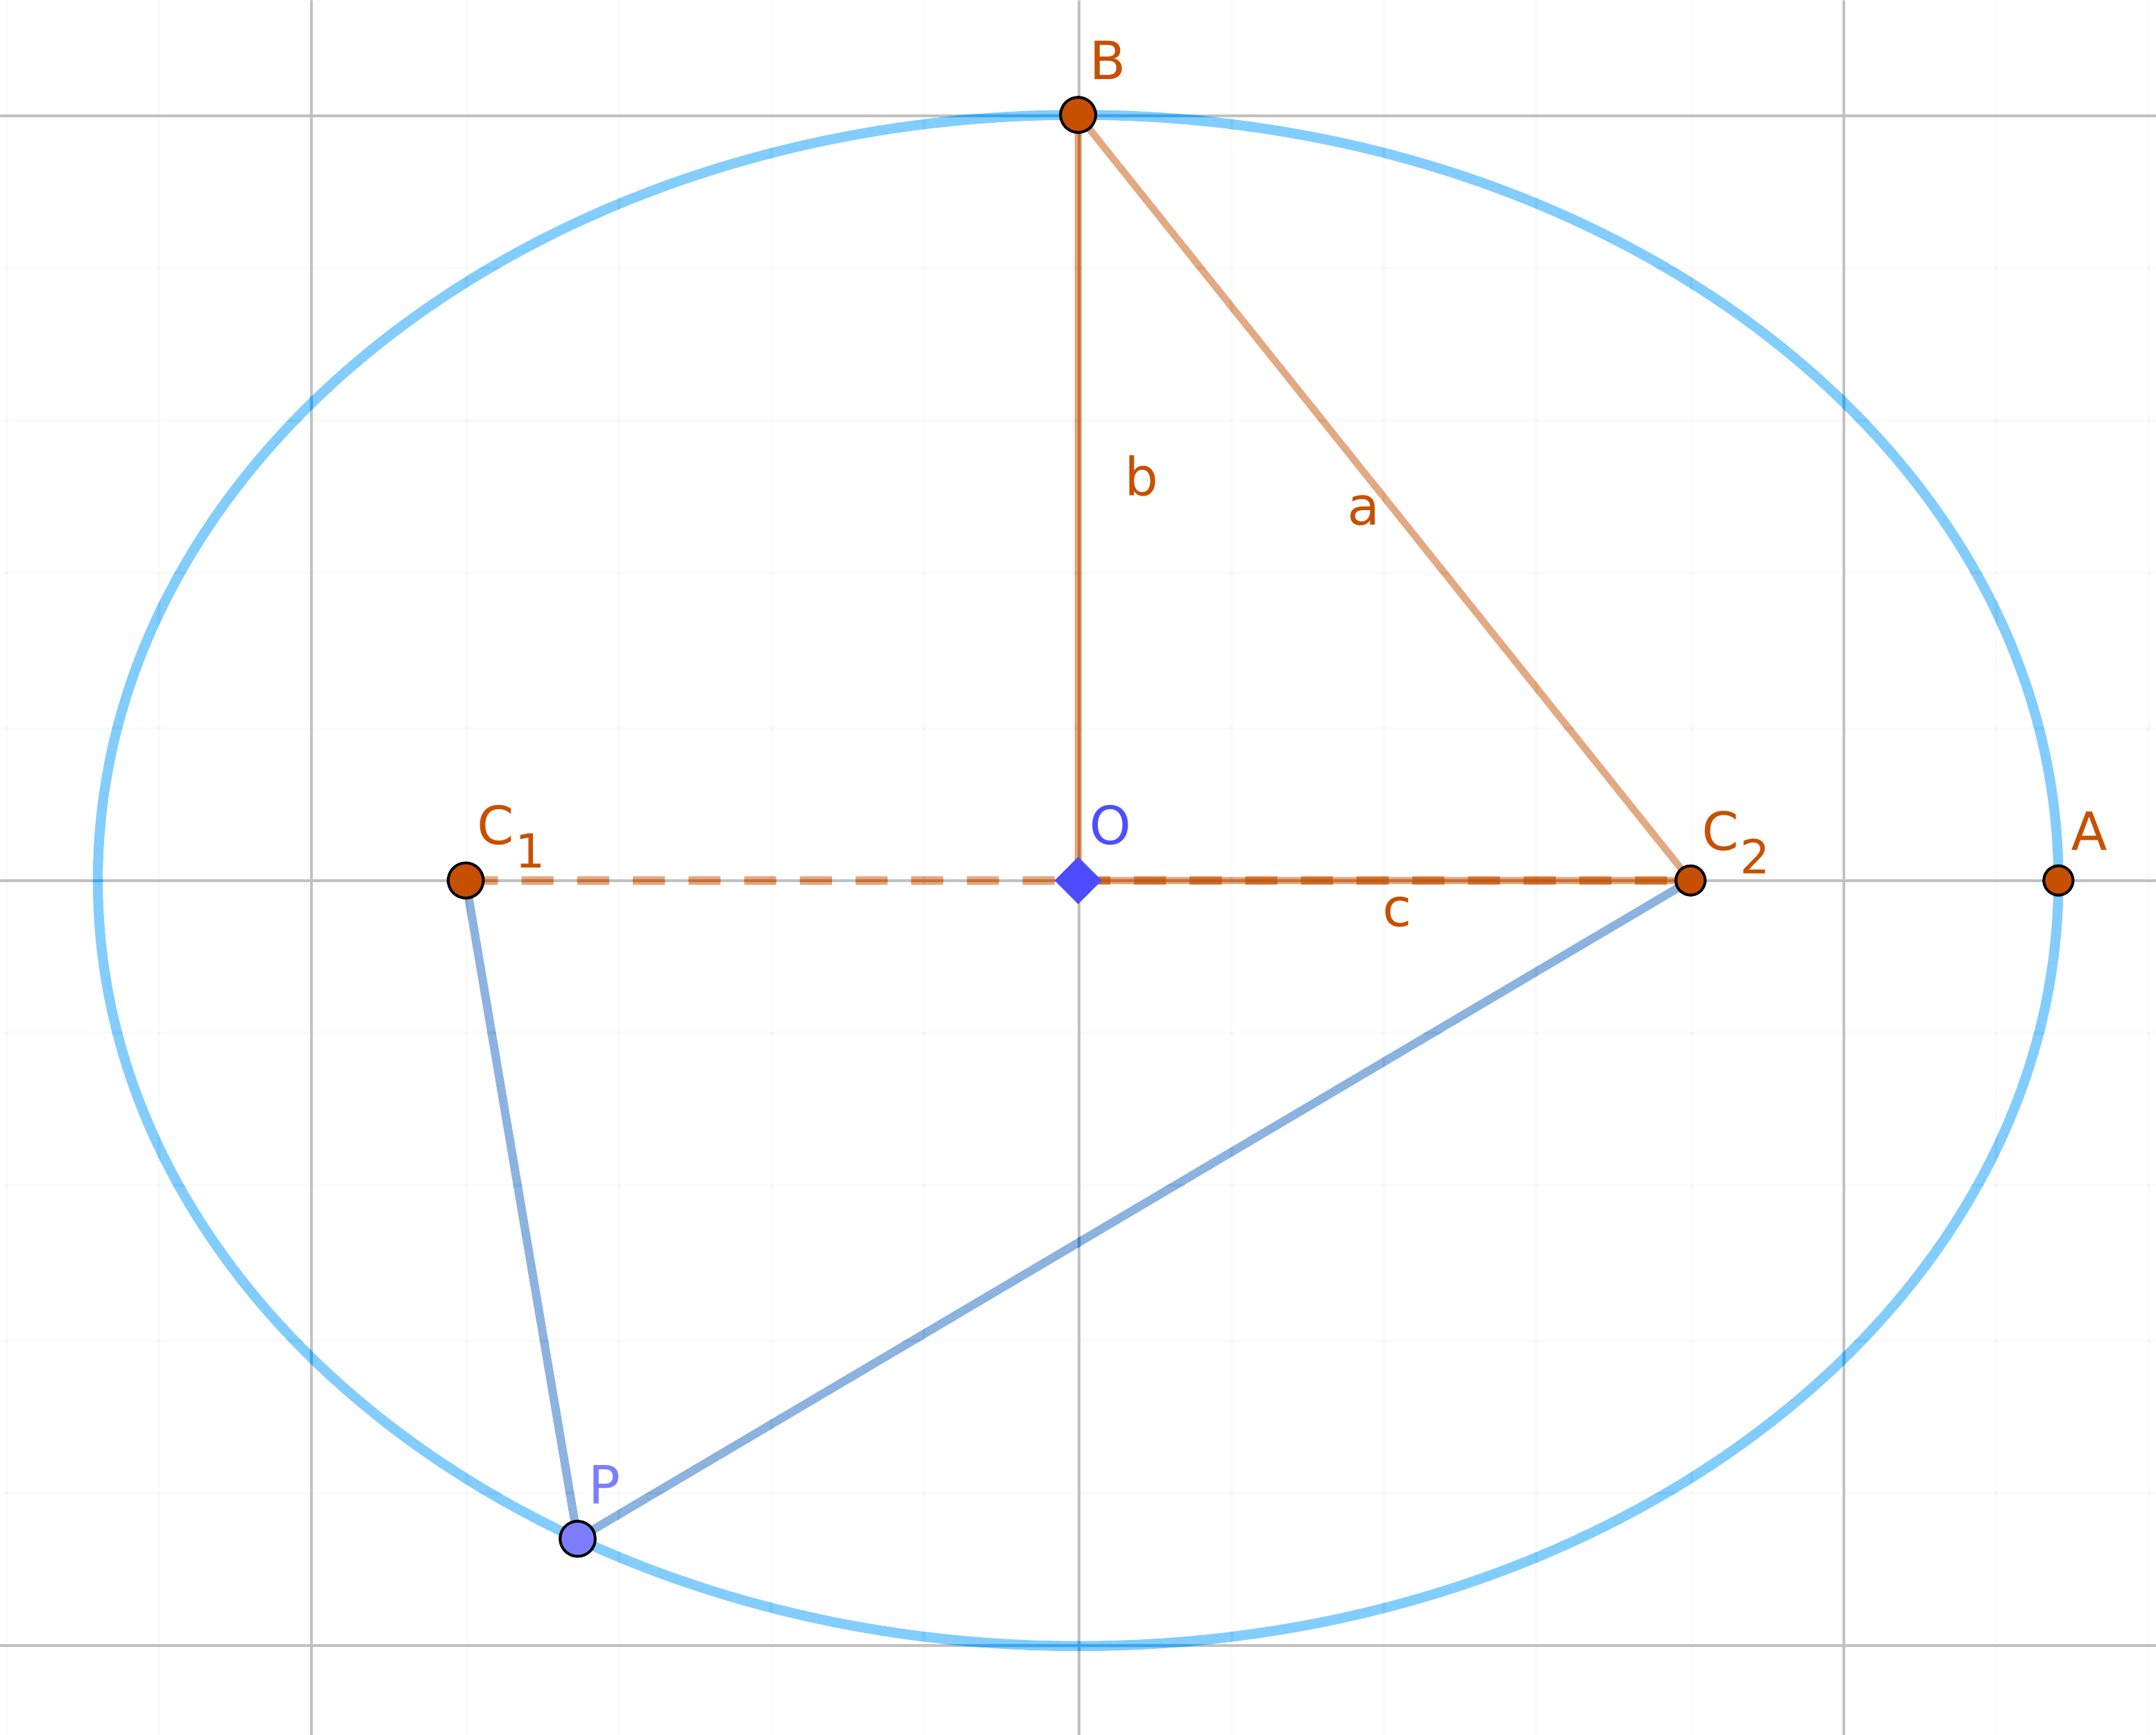
\includegraphics[width=0.75\linewidth]{Images/Ellipse.png}
    \caption{Special points and parameters of an ellipse}
    \label{fig:enter-label}
\end{figure}
An ellipse is a locus of points in a plane whose distances from two focal points in that plane have a constant sum.

Let the focal points be \(C_{1}\ ,\ C_{2}\), and \(O\) be their midpoint, which will be the center of the ellipse.\\ For any point \(P\), \(C_{1}P + C_{2}P = k\).

Line passing through focal points is called the Major Axis, while line passing through the Center and perpendicular to the Major Axis in the plane of the ellipse is called the Minor Axis.

Let ( \(OA = a\) ) be semi-major axis, ( \(OB = b\) ) be semi-minor axis, and ( \(OC = c\) ) be focal distance from center.

Some useful relations are as follows:
\[a = \frac{k}{2}\]
\[a^{2} = b^{2} + c^{2}\]

Since we require each co-ordinate of ellipses separately, we will consider vector equation of ellipse.
\[\vec{r} = a \cdot \cos(\theta)\ \hat{i} + b \cdot \sin(\theta)\ \hat{j} + \ \Vec{O}\]
This is the standard equation of an ellipse with center \(\vec{O}\) and axes along x-axis \& y-axis.

In fact, we can replace standard unit vectors with any set of mutually perpendicular unit vectors to make an ellipse in any orientation anywhere in the 2-D space.
\[\vec{r} = a \cdot \cos(\theta)\ \hat{a} + b \cdot \sin(\theta)\ \hat{b} + \ \Vec{O}\]
These vectors even need not be restricted to 2-D spaces, they can be vectors of any dimensions. We will concern ourselves with Ellipses in 3-D space. This works by making standard ellipse in vector space \(\mathcal{A}\) defined by basis vectors\((\hat{a}\ ,\ \hat{b} )\), then this space is defined as subset of \(\mathcal{X}\) having basis \((\hat{i}\ ,\ \hat{j}\ , \hat{k} )\) by having \((\hat{a}\ ,\ \hat{b} )\) themselves be vectors in \(\mathcal{X}\). Then, the whole ellipse is translated to desired center point \(\vec{O}\). 

Let any vector \(x\hat{i} + y \hat{j} + z\hat{k}\) be
represented as a matrix \(\big[\begin{matrix}x & y & z \end{matrix}\big]\)
\[\begin{bmatrix}r_{x} & r_{y} & r_{z}\end{bmatrix} = a \cdot \cos(\theta)\ 
\begin{bmatrix}a_{x} & a_{y} & a_{z} \end{bmatrix} + \ b \cdot \sin(\theta)\
\begin{bmatrix}b_{x} & b_{y} & b_{z}\end{bmatrix}\]
\[\begin{bmatrix}r_{x} & r_{y} & r_{z}\end{bmatrix} = a
\begin{bmatrix}\cos(\theta)a_{x} & \cos(\theta)a_{y} & \cos(\theta)a_{z}\end{bmatrix} + b
\begin{bmatrix}\sin(\theta)b_{x} & \sin(\theta)b_{y} & \sin(\theta)b_{z}\end{bmatrix}\]
\(\big[\begin{matrix}r_{x} & r_{y} & r_{z}\end{matrix}\big]\) is a single row giving the position of a point at any
\(\theta\). If we were to have a set of discrete values in
\(\lbrack 0,\ 2\pi\rbrack\) at some fixed interval such that \(r\) is
matrix with values corresponding to each value of \(\theta\) in each
row.
\[\begin{bmatrix}
r_{x} & r_{y} & r_{z} \\
\end{bmatrix} = a\begin{bmatrix}
a_{x}\cos(0) & a_{y}\cos(0) & a_{z}\cos(0) \\
 \vdots & \vdots & \vdots \\
 \vdots & \vdots & \vdots \\
 \vdots & \vdots & \vdots \\
a_{x}\cos(2\pi) & a_{y}\cos(2\pi) & a_{z}\cos(2\pi) \\
\end{bmatrix} + b\begin{bmatrix}
b_{x}\sin(0) & b_{y}\sin(0) & b_{z}\sin(0) \\
 \vdots & \vdots & \vdots \\
 \vdots & \vdots & \vdots \\
 \vdots & \vdots & \vdots \\
b_{x}\sin(2\pi) & b_{y}\sin(2\pi) & b_{z}\sin(2\pi) \\
\end{bmatrix}\]

\[\begin{bmatrix}
r_{x} & r_{y} & r_{z} \\
\end{bmatrix} = a\ \begin{bmatrix}
\cos(0) \\
 \vdots \\
 \vdots \\
 \vdots \\
\cos(2\pi) \\
\end{bmatrix}*\begin{bmatrix}
a_{x} & a_{y} & a_{z} \\
\end{bmatrix} + \ b\ \begin{bmatrix}
\sin(0) \\
 \vdots \\
 \vdots \\
 \vdots \\
\sin(2\pi) \\
\end{bmatrix}*\begin{bmatrix}
b_{x} & b_{y} & b_{z} \\
\end{bmatrix}\]

Extracting \(r_{x}\ ,\ r_{y}\ ,\ r_{z}\) , we get one column of the co-ordinate sheets. So, we will one by one repeat process for each individual ellipse and add \(\big[\begin{matrix} O_{x} & O_{y} & O_{z} \\ \end{matrix}\big]\) in the end to shift ellipses to their center.

\hypertarget{the-compromise}{%
\subsection{The Compromise}\label{the-compromise}}

Channel Directrix is the curve that passes through the centers of all
ellipses.

\[D = \frac{F_{1} + F_{2}}{2}\]

Each ellipse we obtain must satisfy the following properties:

\begin{itemize}
\item
  Major Axis must pass through the Focal Points
\item
  Ellipses must be perpendicular to the Directrix of the Channel, i.e.,
  the normal vector of ellipses must be tangential to the directrix. (Both axes
  of ellipse must be normal to the tangent of directrix)
\item
  Major and Minor Axes must be mutually perpendicular
\end{itemize}

Third Property is unnegotiable and must be fulfilled no matter what, for cross-section to be elliptical in the first place, but the first two properties cannot be satisfied simultaneously except in some very special scenarios.

To satisfy both properties, the cross-section must be non-Euclidean, meaning it is bounded by an elliptical disc bent in space such that it passes through both foci and the center. Additionally, it must be normal to both focal curves and the directrix. Unfortunately, this combination of conditions leads us to right in the beginning with all of the complex mathematics.

Therefore, we will accept only one of the properties,

\hypertarget{major-axis-must-always-pass-through-the-focal-points}{%
\subsubsection{Major Axis must always pass through the Focal
Points}\label{major-axis-must-always-pass-through-the-focal-points}}

Let \(\hat{n}\) be a unit vector tangent to the Directrix.

\[\hat{a} = \frac{1}{2}\frac{\begin{bmatrix}
\ \left( \ F_{x}^{2} - F_{x}^{1}\  \right) & \left( \ F_{y}^{2} - F_{y}^{1}\  \right) & \left( \ F_{z}^{2} - F_{z}^{1}\  \right) \\
\end{bmatrix}}{\sqrt{\left( \ F_{x}^{2} - F_{x}^{1}\  \right)^{2}\  + \ \left( \ F_{y}^{2} - F_{y}^{1}\  \right)^{2} + \ \left( \ F_{z}^{2} - F_{z}^{1}\  \right)^{2}}\ }\]

\[\hat{b} = \ \hat{n}\  \times \hat{a}\]

\(\hat{a}\) and \(\hat{n}\) are not necessarily perpendicular to each other, but \(\hat{b}\) is to both. Therefore, at least, the minor axis is always perpendicular to the tangent of the directrix.

\hypertarget{both-axes-must-be-always-perpendicular-to-tangent-of-directrix}{%
\subsubsection{Both axes must be always perpendicular to the tangent of
directrix}\label{both-axes-must-be-always-perpendicular-to-tangent-of-directrix}}

For this we will repeat above steps to find \(\hat{b}\), and then we
will redefine \(\hat{a}\)

\[\hat{a} = \hat{b} \times \hat{n}\]

Now \(\hat{a}\) is perpendicular to both \(\hat{b}\) and
\(\hat{n}\) , who were already perpendicular to each other.
\\
\textit{We will obey ``Major Axis must always pass through the Focal Points'', for having more authenticity of the role of Focal Axes as the Foci of the Cross-sections of the Channel.}

\hypertarget{the-cross-sections}{%
\subsection{The Cross-Sections}\label{the-cross-sections}}
We use \textit{norm()} function to get vector length and divide vector it to make it a unit vector \cite{mathworks_norm}.
\begin{lstlisting}[language=matlab]
t      = 0: 0.01 :2*pi+0.1;
cyl_x  = zeros(size(t'*x));                        % Container matrices for coordinates
cyl_y  = cyl_x;
cyl_z  = cyl_x;

for n=1:size(x,2)
    norm_vec       = [1 tangent_y(n) tangent_z(n)];
    norm_vec       = norm_vec/norm(norm_vec);      % to make it a unit vector
    focal_vec      = [(p(n)-u(n))/2 (q(n)-v(n))/2 (r(n)-w(n))/2];
    minor_vec      = cross(norm_vec,focal_vec);
    
    minor_vec      = minor_vec/norm(minor_vec);
    major_vec      = focal_vec/norm(focal_vec);
    point_vec      = (major(n) * (cos(t)'*major_vec) + minor(n) * (sin(t)'*minor_vec));
 
    % Each column coressponds to a elliptical cross-section
    cyl_x(1:end,n) = point_vec(1:end,1);
    cyl_y(1:end,n) = point_vec(1:end,2);
    cyl_z(1:end,n) = point_vec(1:end,3);
end

varcl = {'norm_vec','major_vec','minor_vec','point_vec','n','varcl'};
clear (varcl{:});

k       = ones(size(t));                       
shift_x = k'*x;                                   % All points in each column
shift_y = k'*y;                                   % will have same displacement
shift_z = k'*z;
cyl_x   = cyl_x + shift_x;
cyl_y   = cyl_y + shift_y;
cyl_z   = cyl_z + shift_z;

\end{lstlisting}

\newpage
\hypertarget{the-rendering}{%
\section{ The Rendering}\label{the-rendering}}
All the code described throughout the document is compiled into one \(.m\) file in sequence and executed in Matlab. \(surf()\) function is used plot the surface \cite{mathworks_surf}. Resultant surface object has several properties that can be modified like \cite{mathworks_surface_properties}
\begin{itemize}
    \item EdgeAlpha (0-1) : Opacity of Edges in Mesh. Set to 0 as dense mesh causes whole figure to black out
    \item FaceColor : Color of the surface. Set to in-built option "interp" that shades a gradient based on z-value
    \item FaceLighting : Defines light source for surface.
    \item SpecularStrength (0-1): Defines Mattness or Gossiness of the surface
    \item AmbientStrength (0-1): Defines strength of ambient light that illuminates from all directions
\end{itemize}
\begin{lstlisting}[language=matlab]
g_cyl= surf(cyl_x,cyl_y,cyl_z); % 
g_cyl.EdgeAlpha             = 0;
g_cyl.FaceColor             = "interp";
g_cyl.FaceAlpha             = 1;
g_cyl.FaceLighting          = "gouraud";
g_cyl.AmbientStrength       = 0.6;
g_cyl.SpecularStrength      = 0.2;

axis equal;
axis auto;
xlabel("x-axis");
ylabel("y-axis");
zlabel("z-axis");
grid on
\end{lstlisting}

Following code is used to make the test data for all the figures thereafter
\begin{lstlisting}[language=matlab]
helix_rad     = 6;
helix_stretch = 10;
x             = 0:0.1:50;
a             = helix_rad*cos(1*x/helix_stretch-pi/4);
b             = helix_rad*sin(1*x/helix_stretch-pi/4);
rad           = (sin(pi*sin(x/8).^2) + cos(3*pi/2*sin(x/7)) + exp((x-5)/35)) + 1;
c             = -1*helix_rad*cos(1.2*x/helix_stretch-pi/4);
d             = -1*helix_rad*sin(1.1*x/helix_stretch-pi/4);
save("curves.txt","x","a","b","x","c","d","rad","-ascii");

\end{lstlisting}

\begin{figure}[h]
    \centering
    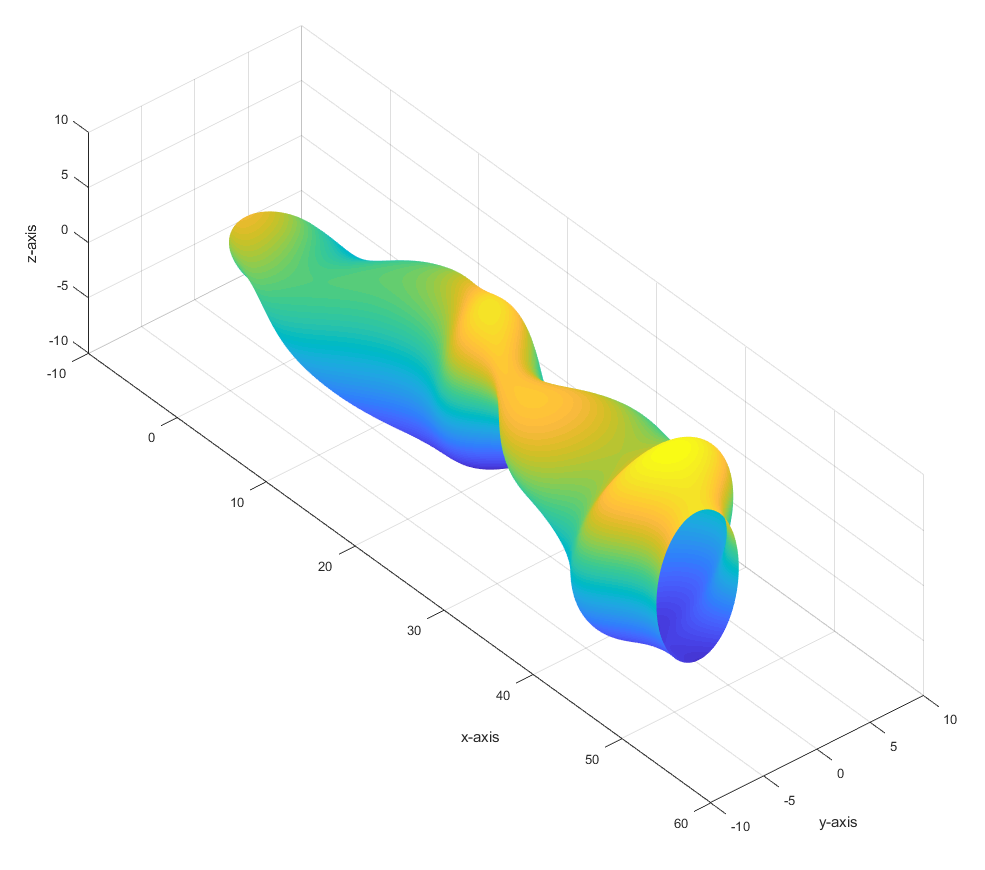
\includegraphics[width=1\linewidth]{Images/Uncharted_Tunnel_Left.png}
    \caption{Rendering of Calculated Mesh}
    \label{Channel with cross-sections}
\end{figure}
%\newpage
\hypertarget{the-plot}{%
\subsection{Cross-sections}\label{the-plot}}

We can further enhance this plot by also incorporating boundaries around cross-sections. To avoid it becoming an incoherent mess, we will select only a few cross-sections that are reasonably far apart from each other.

\begin{lstlisting}[language=matlab]
hold on
cross_density = 15;
g_cross       = plot3(cyl_x(1:end, 1:(1+cross_density):end),...
                      cyl_y(1:end, 1:(1+cross_density):end),...
                      cyl_z(1:end, 1:(1+cross_density):end),...
                      'LineWidth',1);
end
\end{lstlisting}

\begin{figure}[h]
    \centering
    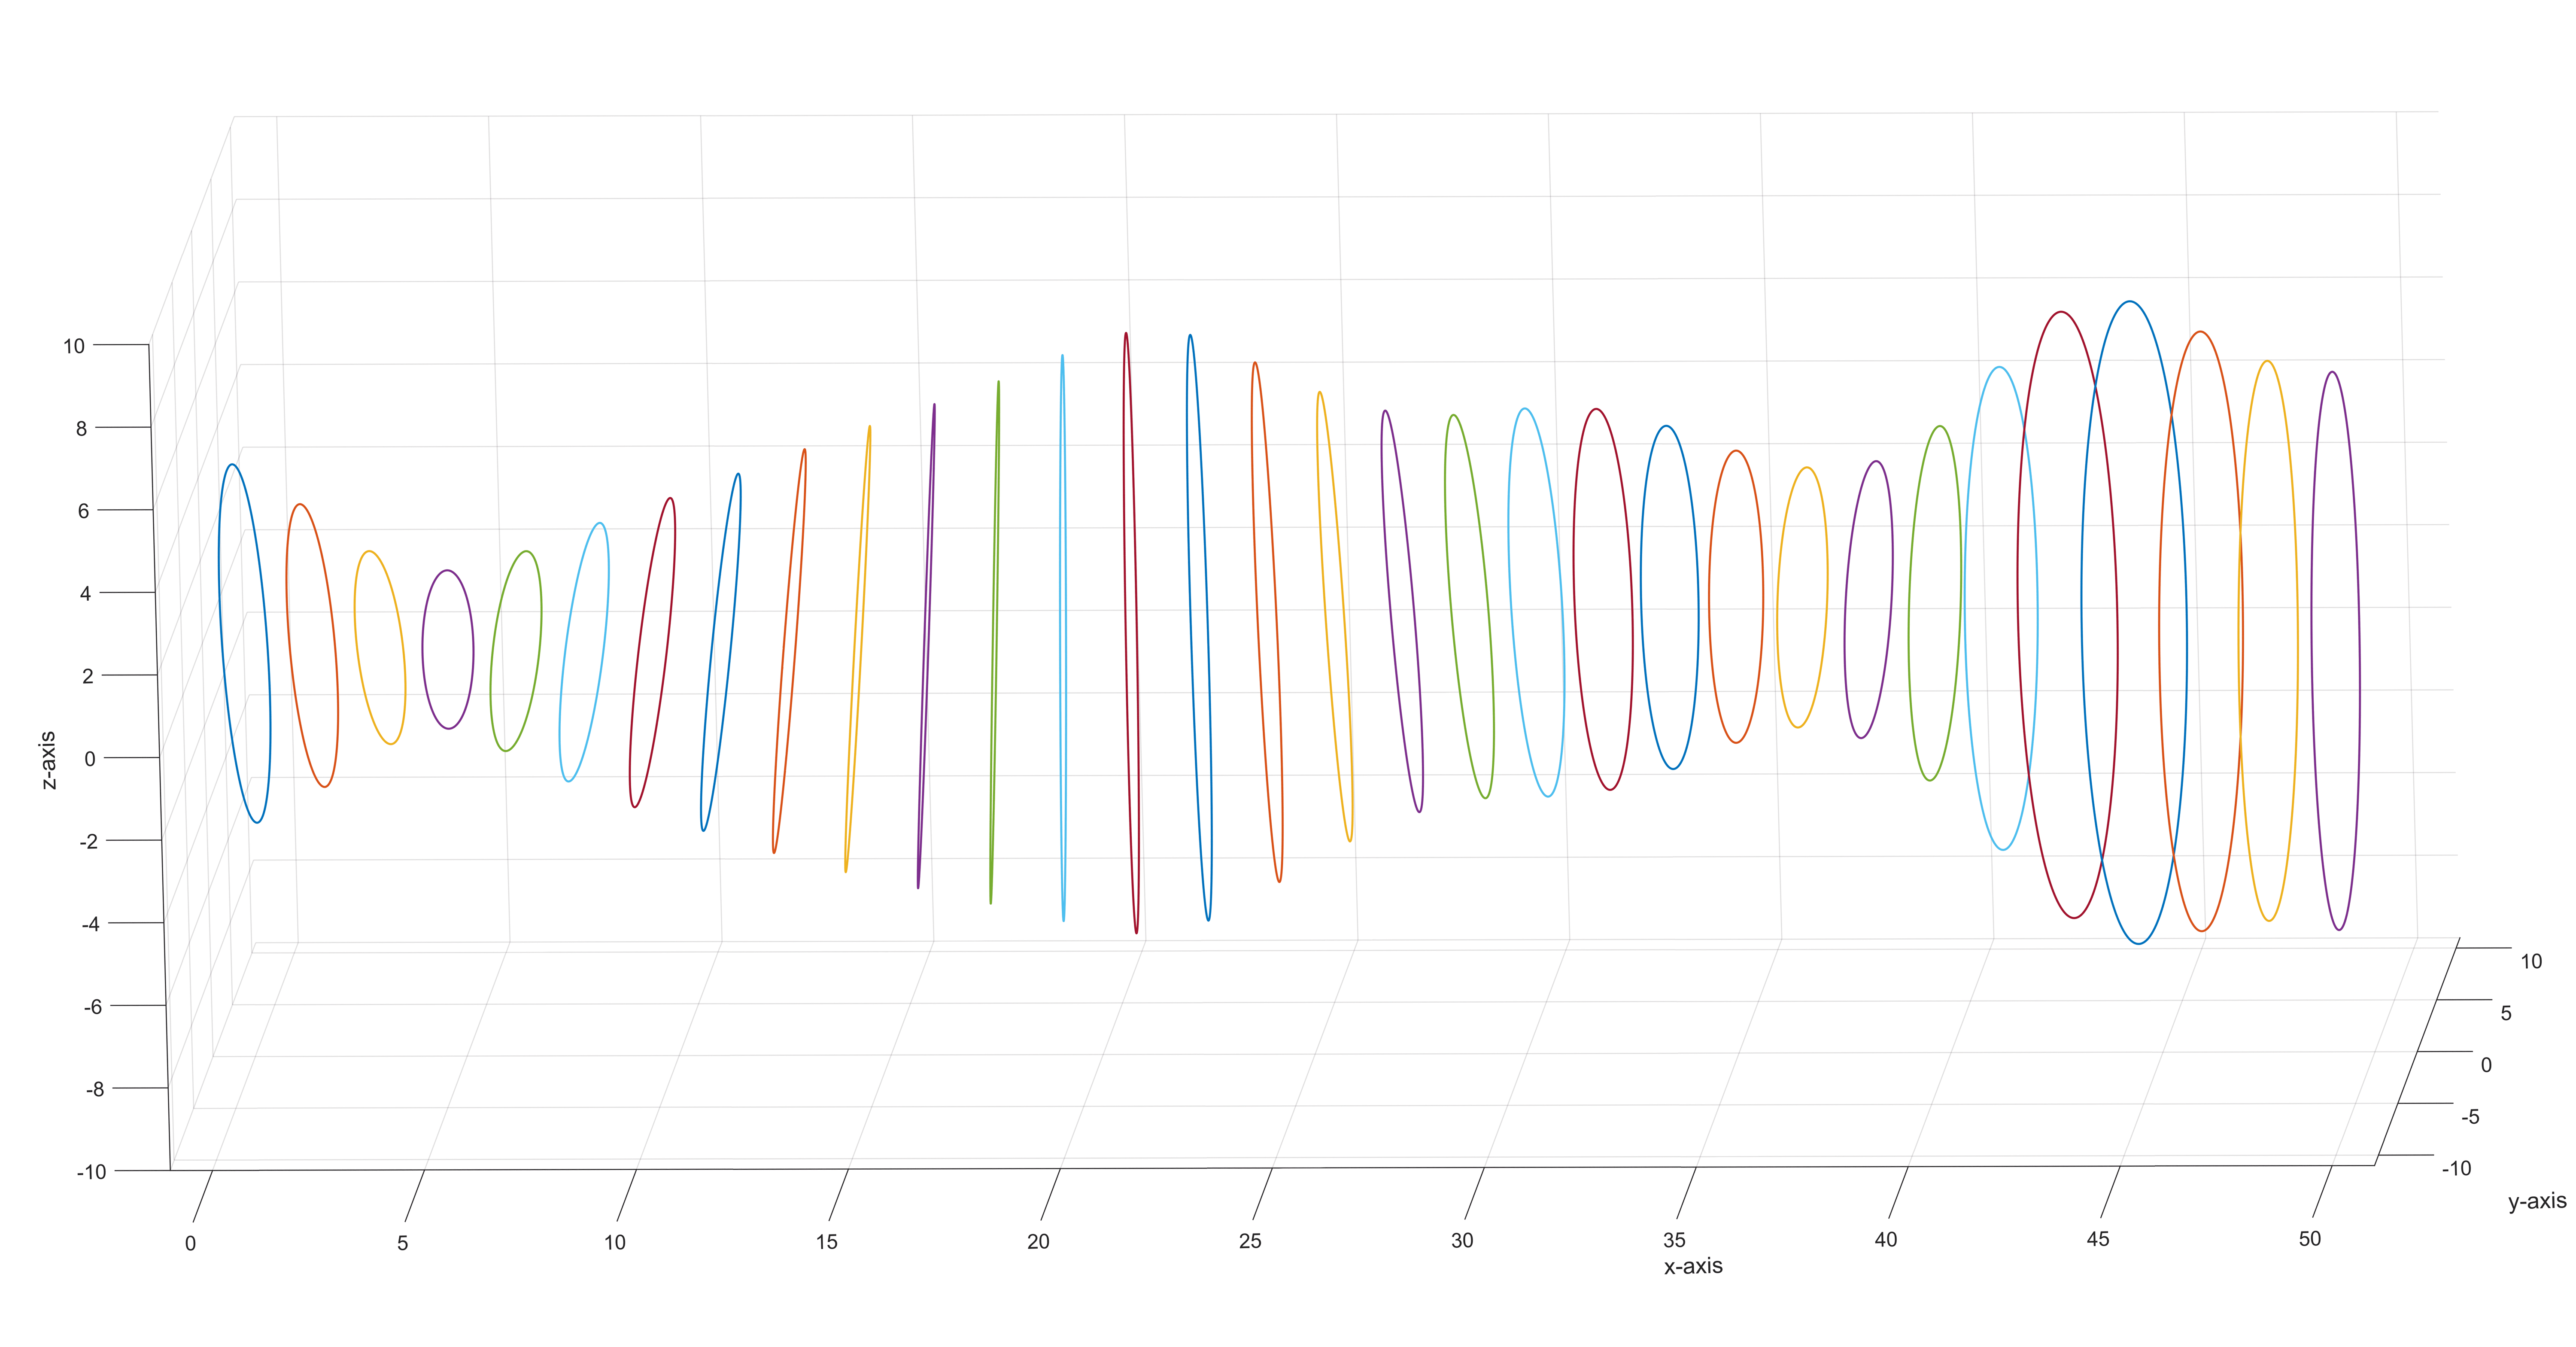
\includegraphics[width=0.8\linewidth]{Images/Skeleton.png}
    \caption{Plots of Cross-sections only}
    \label{fig:enter-label}
\end{figure}

\(plot3\), when given a \(2D\) array (matrix), plots each column as an individual curve \cite{mathworks_plot3}. Therefore, we provide all the rows (complete columns) and select columns at some intervals ( \(1+cross\_density\) ). This gives us \(cyl\_x( 1 : end , 1 : 1+cross\_density : end)\). The term in brackets is the index of elements following the convention of (rows, columns). Ranges can be used to filter out entire rows or columns. A range is defined as ‘Start : Step : End', where Step is 1 by default if not mentioned.
\begin{figure}[h!]
    \centering
    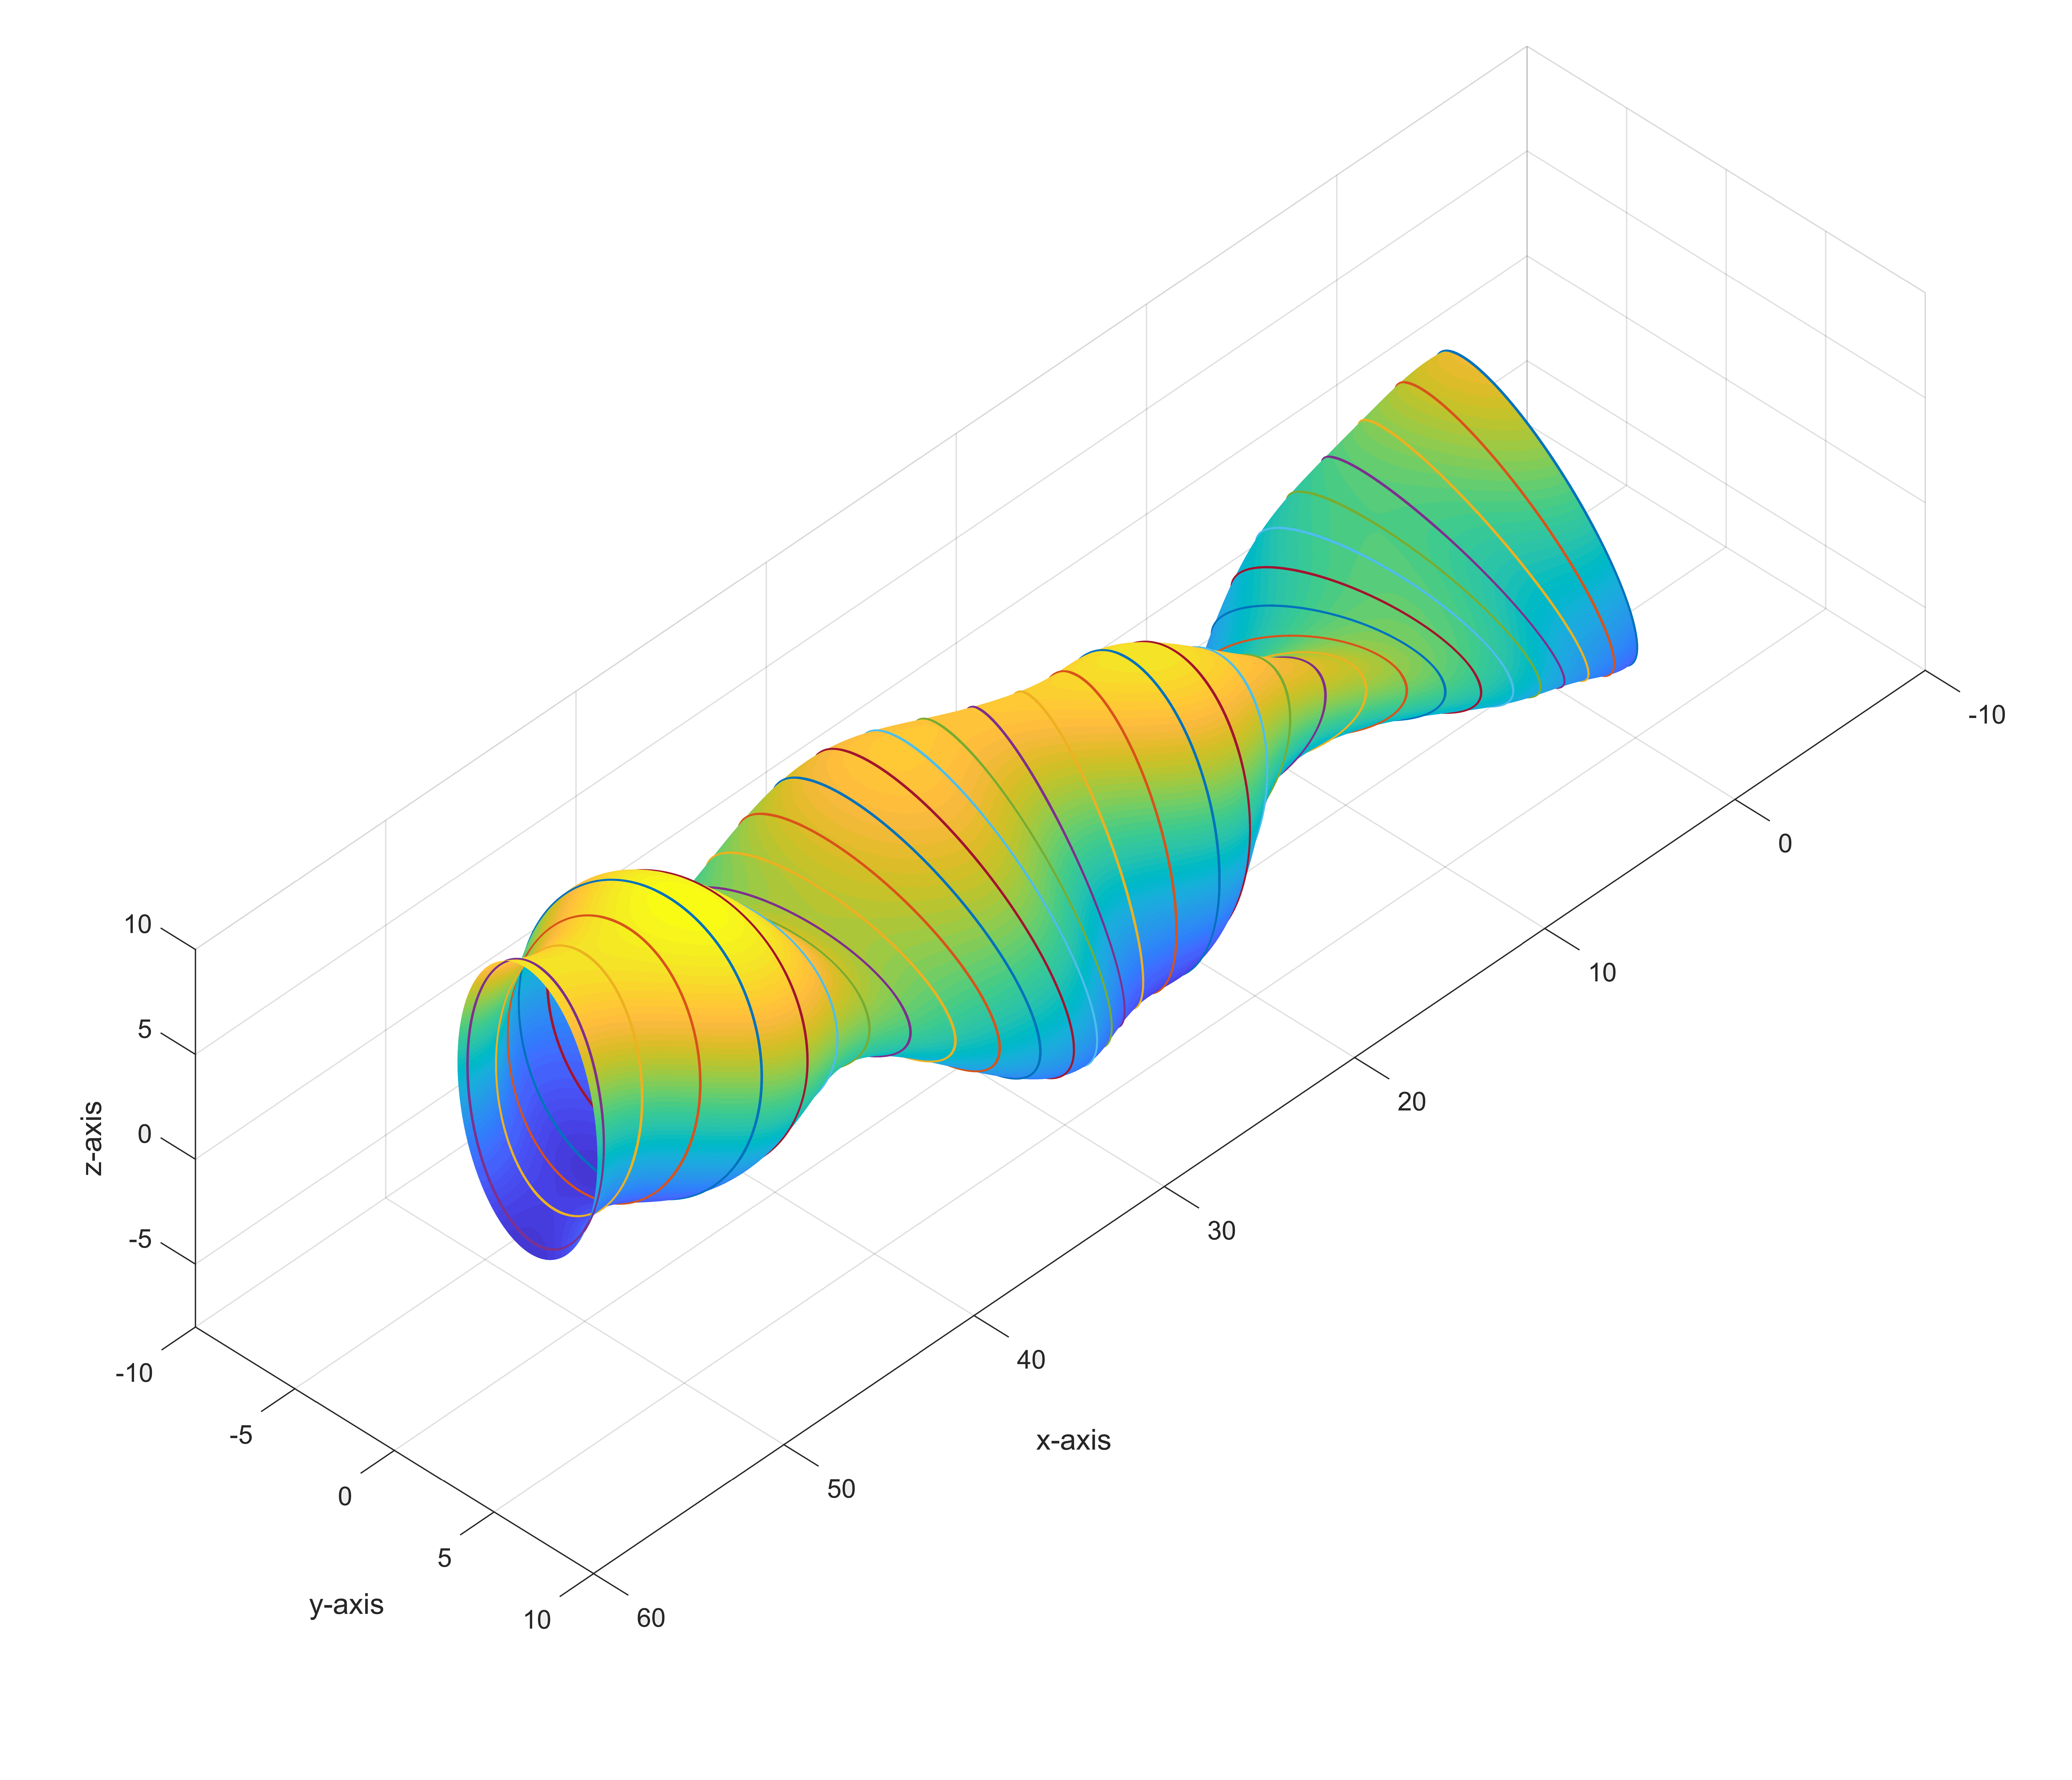
\includegraphics[width=0.75\linewidth]{Images/Charted_Tunnel_Right.png}
    \caption{Channels with sparsely marked cross-sections}
\end{figure}

\subsection{Shadows}
While we’re on the topic, why not also add shadows to enhance the sense of perspective and orientation? This can be achieved by simply plotting the surface again, but with one of the axes almost scaled to zero and shifted to the desired location.

The resulting figure would essentially be a projection onto the plane of the unscaled axes. We don’t scale the axes to exactly zero (which would work just fine), because the minuscule depth of the figure would make the shadows in more overlapping regions darker if we made them translucent.

\begin{lstlisting}[language=matlab]
shadow_xy = surf(cyl_x,cyl_y,cyl_z*0.01-15);
shadow_xz = surf(cyl_x,cyl_y*0.01+15,cyl_z);
shadow_yz = surf(cyl_x*0.01-15,cyl_y,cyl_z);

shadowEdgeAlpha=0;
ShadowColor=[0,0,1];
ShadowAlpha=0.15;

shadow_xy.EdgeAlpha             = shadowEdgeAlpha;
shadow_xy.FaceColor             = ShadowColor;
shadow_xy.FaceLighting          = "gouraud";
shadow_xy.FaceAlpha             = ShadowAlpha;

shadow_xz.EdgeAlpha             = shadowEdgeAlpha;
shadow_xz.FaceColor             = ShadowColor;
shadow_xz.FaceLighting          = "gouraud";
shadow_xz.FaceAlpha             = ShadowAlpha;

shadow_yz.EdgeAlpha             = shadowEdgeAlpha;
shadow_yz.FaceColor             = ShadowColor;
shadow_yz.FaceLighting          = "gouraud";
shadow_yz.FaceAlpha             = ShadowAlpha;
\end{lstlisting}
\newpage
\begin{figure}[h]
    \centering
    \includegraphics[width=1\linewidth]{Images/Shadowed_Tunnnel.png}
    \caption{Channels with cross-sections and shadows}
\end{figure}

\newpage
\bibliographystyle{unsrt}
\bibliography{references}

\textbf{All figures except figure 1 are made by the Author only, with MATLAB and GeoGebra}\\
Complete Code available at \url{https://github.com/Rajnoor-Brar/Ellipsoidal-Channel}
\end{document}